

\documentclass[a4paper,12 pt]{article}

\usepackage[margin=2.5cm]{geometry} % margin
\usepackage{multicol} % multiple columns
\usepackage{pgfplots} % graphs
\usepackage{graphicx}
\usepackage{float}
\usepackage{caption} % figure and subfigure
\usepackage{subfig}
\usepackage{verbatim}
\usepackage{booktabs} % toprule, midrule
\usepackage[colorlinks=true, urlcolor=black, linkcolor=black, citecolor=black, filecolor=black]{hyperref} % hyperref
\usepackage{enumerate}

\usepackage[english]{babel} % language

\usepackage{amsmath} % maths packages
\usepackage{amssymb}
\usepackage{amsthm}
\usepackage{nicefrac}


\renewcommand*\contentsname{Inhaltverzeichnis} % inhaltverzeichnis statt Contents

\setlength{\parindent}{0cm} % remove indentation

%\numberwithin{equation}{section} % equation number


%%%%%%%%%%%%%%%% HEADING

\usepackage{fancyhdr} % HEADING
\pagestyle{fancy}
\lhead{Gioele Zardini}
\chead{Vision Algorithms for Mobile Robotics}
\rhead{HS 2017}
\renewcommand{\headrulewidth}{0.4pt}
%\renewcommand{\footrulewidth}{0.4pt}

%%%%%%%%%%%%%%%%


%%%%%%%%%%%%%%%% NEW COMMANDS

\newcommand{\pt}[1]{\frac{\text{d}}{\text{d} t}#1}

\theoremstyle{definition}
\newtheorem{bsp}{Example}
\theoremstyle{remark}
\newtheorem*{bmk}{Remark}
\theoremstyle{definition}
\newtheorem*{lsg}{Solution}
\theoremstyle{definition}
\newtheorem{df}{Definition}
\theoremstyle{definition}
\newtheorem{satz}{Theorem}
\theoremstyle{remark}
\newtheorem*{knt}{Kontrolle}

\theoremstyle{definition}
\newtheorem*{solution}{Solution}


%%%%%%%%%%%%%%%% 


%%%%%%%%%%%%%%%% TIKZ

\usepackage{tikz}

\usepackage{pgfplots} % graphs
\usetikzlibrary{positioning,intersections, hobby, patterns, calc, decorations.pathmorphing, decorations.markings, shadows}


\tikzstyle{blockDyn} = [draw, rectangle, minimum height=2.5em, minimum width=3.5em, align=center, inner sep=10pt, thick, fill=white, copy shadow={draw=black,fill=black,opacity=1,shadow xshift=0.5ex,shadow yshift=-0.5ex}]
\tikzstyle{blockAlg} = [draw, rectangle, minimum height=1.5em, minimum width=2.5em, align=center, inner sep=10pt, thick]
\tikzstyle{sum} = [draw,circle]
\tikzstyle{arrow} = [thick]
\tikzstyle{input} = [coordinate]
\tikzstyle{output} = [coordinate]
\tikzstyle{pinstyle} = [pin edge={to-,thin,black}]

%%%%%%%%%%%%%%%%







\begin{document}

%%%%%%%%%%%%%%%%
\begin{huge}{\textbf{Lecture Summary}}\end{huge} \\
\setcounter{section}{1}
\setcounter{secnumdepth}{4}
%%%%%%%%%%%%%%%%
\setcounter{section}{1}
\setcounter{subsection}{0}

\section*{Lecture 01: Introduction}
\begin{df}
\textbf{Computer Vision}: Automatic extraction of meaningful information from images and videos.
\begin{itemize}
\item Semantic information: meaning of objects.
\item Geometric information: shapes.
\end{itemize}
\end{df}
\subsection*{Vision in Humans}
Vision is the most powerful sense:
\begin{itemize}
\item Retina $\approx 1000mm^2$.
\item Contains 130 million \textbf{photoreceptors}
\item $3\text{GBytes}/s$ information flow, would need 500 Megapixel camera (8 Megapixel and range 15 degrees)
\end{itemize}
Why hard? 
\begin{itemize}
\item only numbers, viewpoint variations, illumination challenges, motion, intra-class variations, scale and shape ambiguities
\end{itemize}
\textbf{Origin:} L.G. Roberts, MIT, 1963 , Solids Perception.
\subsection*{Visual Odometry (VO)}
\begin{df}
VO is the process of incrementally estimating the pose of the vehicle by examining the changes that motion induces on the images of its onboard cameras
\end{df}
\subsubsection*{Why VO?}
\begin{itemize}
\item $\neq$ Wheel Odometry, VO \textbf{not affected} by wheel slippage and adverge conditions in general.
\item More accurate. Relative position error 0.1-2 \%.
\item Crucial for flying, walking and underwater robots.
\end{itemize}
\subsubsection*{Assumptions}
\begin{itemize}
\item \textbf{Sufficient illumination},
\item \textbf{dominance of static scene} over moving objects,
\item \textbf{enough texture} to allow apparent motion,
\item \textbf{sufficient scene overlap} between consecutive frames.
\end{itemize}
\subsubsection*{History}
\begin{itemize}
\item 1980: NASA, Moraveck, Mars Rovers, sliding camera.
\item 1980-2000: NASA: mission to mars.
\item 2004: David Nister: Visual Odometry paper.
\end{itemize}
\subsubsection*{VO vs VSLAM vs SFM}
\begin{equation*}
\text{SFM}>\text{VSLAM}>\text{VO}.
\end{equation*}
\textbf{Structure From Motion (SFM)}: more general than VO, tackles the problem of 3D reconstruction and 6DOF pose estimation from \textbf{unordered image sets}. \\
$\rightarrow$ VO focuses on estimating 3D motion \textbf{sequentially} and in \textbf{real time}. \\
\textbf{Visual Simultaneous Localization And Mapping (VSLAM)}:
\begin{itemize}
\item focus on \textbf{globally consistent} estimation.
\item $\text{VSLAM}=\text{VO}+\text{loop detection} +\text{graph optimization}$.
\item Tradeoff between performance and consistency, simplificity of implementation.
\item VO doesn't need to keep track of all previous history of the camera. Good for real-time.
\end{itemize}
\subsubsection*{Working Principle:}
\begin{enumerate}[1.]
\item Compute the relative motion $T_k$ from images $I_{k-1}$ to image $I_k$
\begin{equation}
T_k=\begin{pmatrix}
R_{k,k-1}&t_{k,k-1}\\
0&1
\end{pmatrix}.
\end{equation}
\item Concatenate them to recover full trajectory
\begin{equation}
C_n=C_{n-1}\cdot T_n
\end{equation}
\item An optimization over the last $m$ poses can be done to refine locally the trajectory (Pose-Graph or Bundle Adjustment).
\end{enumerate}
\subsubsection*{Direct Image Alignment}
$\rightarrow$ The whole problem is a \textbf{minimization} of the \textbf{per-pixel intensity difference}
\begin{itemize}
\item Dense: $\approx$ 300'000 pixels.
\item Semi-Dense: $\approx$ 10'000 pixels.
\item Sparse: $\approx$ 2'000 pixels. (100-200 features x 4x4 patch).
\end{itemize}
\subsubsection*{VO Flowchart}
VO computes the camera path incremental, pose per pose
\begin{enumerate}
\item Image sequence,
\item Feature detection,
\item Feature matching (tracking)
\item Motion estimation (2D-2D,3D-3D,3D,2D),
\item Local optimization.
\end{enumerate}
\newpage 
\section*{Lecture 02: Image Formation}
\subsection*{How to Form an Image}
Placing a film in front of an object and illuminating it, the light is then reflected on the film. Not \textbf{reasonable} image! The rays don't converge in the same point, unsharp, blur.
\subsubsection*{Pinhole Camera}
Adding a barrier with a pinhole $\rightarrow$ camera obscura:
\begin{itemize}
\item Opening is the \textbf{aperture}.
\item Reduces blurring.
\item \textbf{ideal pinhole}: only one ray of light reaches each point on the film. Bigger aperture, blurry image.
\end{itemize}
Why not as small as possible? Diffraction effects as we near the wavelenth and less light gets through.
\subsubsection*{Converging Lens}
\begin{itemize}
\item Rays passing through the \textbf{Optical Center} are not deviated.
\item All rays parallel to the \textbf{Optical Axis} converge at the \textbf{Focal point}
\end{itemize}
Using similar triangles and Figure \ref{fig:focal} one gets
\begin{equation}
\begin{split}
\frac{B}{A}&=\frac{e}{z} \text{ and}\\
\frac{B}{A}&=\frac{e-f}{f}=\frac{e}{f}-1.\\
\end{split}
\end{equation}
Toghether we get the \textbf{thin lens equation}.
\begin{equation}
\frac{e}{f}-1=\frac{e}{z}
\end{equation}
\begin{figure}[h!]
\begin{center}
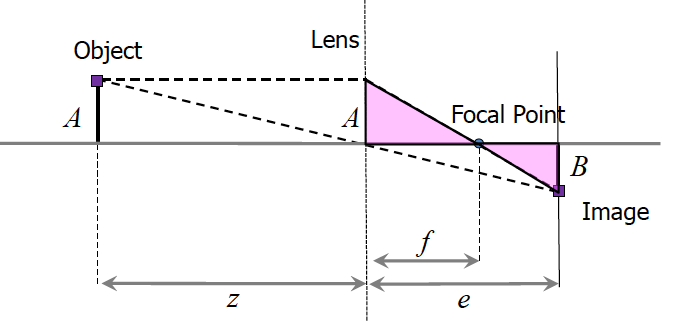
\includegraphics[scale=0.5]{pics/focal}
\caption{Thin lens \label{fig:focal}}
\end{center}
\end{figure}
\begin{bmk}
\
\begin{itemize}
\item Any object point satisfying this equation is in \textbf{focus}.
\item $z>>f$: 
\begin{equation}
\frac{1}{f}=\frac{1}{e} \Rightarrow f \approx e.
\end{equation}
$\rightarrow$ we need to adjust the image plane such that objects at infinity are in focus, namely
\begin{equation}
\frac{h'}{h}=\frac{f}{z} \Rightarrow h'=\frac{f}{z}h.
\end{equation}
The dependence of the apparent size of the object on its depth is known as \textbf{perspective}.

\end{itemize}
\end{bmk}
\subsubsection*{In Focus and Blur Circle}
\begin{itemize}
\item There is a specific distance from the lens at which world points are in focus in the image.
\item Other points project to a \textbf{blur circle} in the image with radius
\begin{equation}
R=\frac{L\delta }{2e}
\end{equation}
$\rightarrow$ a minimal pinhole gives minimal $R$ and\\
$\rightarrow$ $R$ should remain smaller than image resolution.
\end{itemize}
\subsubsection*{Projective Geometry}
\begin{itemize}
\item Straight lines are still straight.
\item Length and angles are lost.
\item Parallel lines in the world intersect in the image as a \textbf{vanishing point}.
\item Parallel planes in the world intersect in the image at a \textbf{vanishing line}. 
\end{itemize}
\subsection*{Other Parameters}
\subsubsection*{Focus and Depth of Field}
\begin{itemize}
\item DOF is the distance between the nearest and farthest objects in a scene that appear acceptably sharp.
\item Decrease in sharpness is gradual on each side of the focused distance.
\item Smaller aperture increases the range in which the object appears in focus but reduces the light.
\item As $f$ gets smaller: \textbf{wide angle} image.
\item As $f$ gets bigger: \textbf{narrow angle} image.
\end{itemize}
With Figure \ref{fig:wide}, one can compute the \textbf{field of view}
\begin{figure}[h!]
\begin{center}
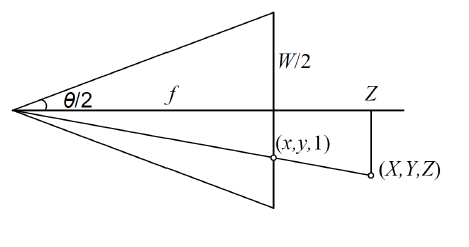
\includegraphics[scale=0.5]{pics/wide}
\caption{Scheme for angles. \label{fig:wide}}
\end{center}
\end{figure}
\begin{equation}
\tan\left( \frac{\theta}{2}\right)=\frac{W}{2f} \Rightarrow f=\frac{W}{2}\left[ \tan \left( \frac{\theta}{2}\right)\right]^{-1}
\end{equation}
$\rightarrow$ smaller FOV = larger focal length.
\subsection*{Digital Camera}
Instead of using a film we use a sensor array and we convert informations in numbers (e.g. $[0,255]$ for 8 bytes), as in Figure \ref{fig:procedure_one}.
\begin{figure}[h!]
\begin{center}
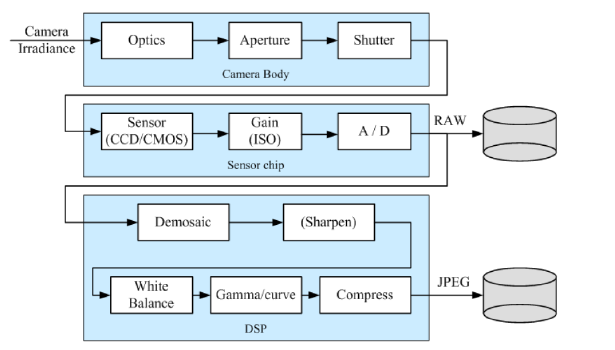
\includegraphics[scale=0.5]{pics/procedure}
\caption{Procedure digital cameras. \label{fig:procedure_one}}
\end{center}
\end{figure}
\subsubsection*{Color Sensing}
\begin{itemize}
\item Byer pattern (1976) places green filters over half of the sensors and red and blue over remaining ones. Humans are more sensintive to high frequency detail in luminance than chrominance.
\item Estimate missing components from neighboring values: \textbf{demosaicing}
\end{itemize}
\subsection*{Perspective Camera Model}
The procedure reads
\begin{enumerate}
\item Change of coordinates from 3D world to adapted frame.
\item Projection from the camera frame to the image plane.
\item Change in pixel.
\end{enumerate}
\begin{figure}[h!]
\begin{center}
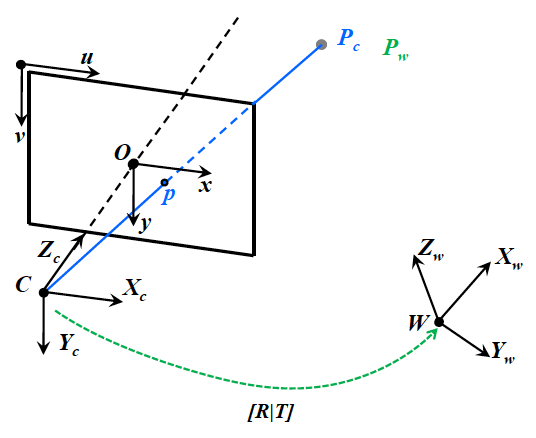
\includegraphics[scale=0.5]{pics/perspective}
\caption{Frames. \label{fig:perspective}}
\end{center}
\end{figure}
\subsubsection*{Perspective Projection}
We use the notation from euclidean to homogeneous:
\begin{equation}
\underbrace{\begin{pmatrix}
u \\
v\\
w
\end{pmatrix}}_{Homog.}\rightarrow 
\underbrace{\begin{pmatrix}
u/w \\
v/w\\
1
\end{pmatrix}}_{Eucl.}
\end{equation}
From similar triangles and Figure \ref{fig:proj} one gets
\begin{equation}
\begin{split}
\frac{x}{f}&=\frac{X_c}{Z_c} \Rightarrow x=\frac{fX_c}{Z_c}\\
\frac{y}{f}&=\frac{Y_c}{Z_c} \Rightarrow y=\frac{fY_c}{Z_c}
\end{split}
\end{equation}

\begin{figure}[h!]
\begin{center}
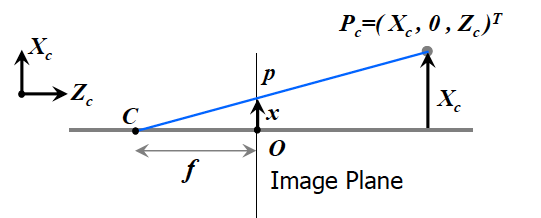
\includegraphics[scale=0.5]{pics/proj}
\caption{Figure for perspective projection. \label{fig:proj}}
\end{center}
\end{figure}
\subsubsection*{Pixel Coordinates}
From local image plane coords $(x,y)$ to the pixel coords $(u,v)$:
\begin{equation}
\begin{split}
u&=u_0+k_ux \Rightarrow u=u_0+\frac{k_ufX_c}{Z_c}\\
v&=v_0+k_ux \Rightarrow v=v_0+\frac{k_vfX_c}{Z_c},
\end{split}
\end{equation}
which expressed in matrix form reads
\begin{equation}
\begin{pmatrix}
\lambda u\\
\lambda v\\
\lambda 
\end{pmatrix}=\begin{pmatrix}
\alpha _u&0&u_0\\
0&\alpha_v &v_0 \\
0&0&1
\end{pmatrix}\cdot \begin{pmatrix}
X_c\\
Y_c\\
Z_c
\end{pmatrix}=K\begin{pmatrix}
X_c\\
Y_c\\
Z_c
\end{pmatrix},
\end{equation}
with $\alpha _u,v$ focal lengths and $K$ \textbf{calibration matrix}. At the end, it holds
\begin{equation}
\lambda \cdot \begin{pmatrix}
u\\
v\\
v
\end{pmatrix}=\underbrace{(K)}_{3\times 3,\ intrinsic}\cdot \underbrace{(\mathbb{I}_{3\times 3}|0)}_{3\times 4}\cdot \underbrace{\begin{pmatrix}
 R&\vec{t} \ \\
 0&1
\end{pmatrix}}_{4\times 4, \ extrinsic}\cdot \begin{pmatrix}
X_w\\
Y_w\\
Z_w
\end{pmatrix}.
\end{equation}
\subsection*{Lens Distortion}
\subsubsection*{Radial Distortion}
This is a transformation from ideal to distorted coordinates. For most lenses, one writes
\begin{equation}
\begin{pmatrix}
u_d\\
v_d
\end{pmatrix}=(1+k_1r^2)\cdot \begin{pmatrix}
 u-u_0\\
 v-v_0
 \end{pmatrix}+\begin{pmatrix}
u_0\\
v_0
\end{pmatrix},
\end{equation}
with
\begin{equation}
r^2=(u-u_0)^2+(v-v_0)^2.
\end{equation}
\newpage
\section*{Lecture 03: Image Formation 2}
\subsection*{Pose determination from $n$ Points (PnP) Problem}
We assume we know the camera intrinsic parameters. Given known 3D landmarks in the world and their image correspondence in the camera frame, determine the 6DOF pose of the camera in the world frame. \textbf{Where is the camera?}
\begin{itemize}
\item Given 1 point: $\infty$ solutions.
\item Given 2 points: $\infty$ \textit{bounded} solutions.
\item Given 3 \textbf{non collinear} points: Finitely many (up to 4) solutions.
\item Given 4 points: unique solution.
\end{itemize}
With 3 points one has the Carnot's theorem
\begin{equation}
s_{1,2,3}^2=L_{B,A,A}^2+L_{C,C,B}^2-2L_{B,A,A}L_{C,C,B}\cos(\theta_{BC,AC,AB})
\end{equation}
In general, $n$ independent polynomials with $n$ unknowns, can have no more solution than the product of their degrees: here 8. \\
$\rightarrow$ fourth point to \textbf{disambiguate} the solutions! By defining $x=\frac{L_B}{L_A}$ we can reduce the system to a $4^{th}$ order equation
\begin{equation}
G_0+G_1x+G_2x^2+G_3x^3+G_4x^4=0.
\end{equation}
This applies to camera pose estimation from known $3D-2D$ correspondences (e.g. hololens).
\subsection*{Camera Calibration}
Determine \textbf{intrinsic} and \textbf{extrinsic} parameters of the camera model. \\
\textit{Tsai, 1987}: Measure the 3D position of more than 6 points on a 3D calibration target and the 2D coordinates of theis projection.
\subsubsection*{Direct Linear Transform}
\begin{equation}
\begin{split}
\text{image point}=\tilde{p}&=\begin{pmatrix}
\tilde{u}\\
\tilde{v}\\
\tilde{w}
\end{pmatrix} = \lambda \begin{pmatrix}
 u\\
 v\\
 1
 \end{pmatrix}=K[R|T]\cdot \begin{pmatrix}
 X_w\\
 Y_w\\
 Z_w\\
 1
 \end{pmatrix}\\
 &=\begin{pmatrix}
\alpha_u &0&0\\
0&\alpha_v &\nu_0\\
0&0&1
\end{pmatrix}\cdot \begin{pmatrix}
 r_{11}&r_{12}&r_{13}&t_1\\
 r_{21}&r_{22}&r_{23}&t_2\\
 r_{31}&r_{32}&r_{33}&t_3
 \end{pmatrix}\cdot \begin{pmatrix}
 X_w\\
 Y_w\\
 Z_w\\
 1
 \end{pmatrix}\\
\textit{assuming indep. elements} \qquad &=\underbrace{\begin{pmatrix}
 m_{11}&m_{12}&m_{13}&m_{14}\\
 m_{21}&m_{22}&m_{23}&m_{24}\\
 m_{31}&m_{32}&m_{33}&m_{34}
 \end{pmatrix}}_{M}\cdot \begin{pmatrix}
 X_w\\
 Y_w\\
 Z_w\\
 1
 \end{pmatrix}\\
 &=\begin{pmatrix}
m_1^T\\
m_2^T\\
m_3^T
\end{pmatrix}\cdot \underbrace{\begin{pmatrix}
 X_w\\
 Y_w\\
 Z_w\\
 1
 \end{pmatrix}}_{P}.
 \end{split}
\end{equation}
It follows
\begin{equation}
\begin{split}
u&=\frac{\tilde{u}}{\tilde{w}}=\frac{m_1^T\cdot P}{m_3^T\cdot P}\\
v&=\frac{\tilde{v}}{\tilde{w}}=\frac{m_2^T\cdot P}{m_3^T\cdot P}
\end{split}
\end{equation}
and hence
\begin{equation}
\begin{split}
(m_1^T-u_im_3^T)\cdot P_i&=0\\
(m_2^T-v_im_3^T)\cdot P_i&=0.
\end{split}
\end{equation}
Rearranging the terms you have
\begin{equation}
\begin{pmatrix}
P_1^T &0^T&-u_1P_1^T\\
0^T&P_1^T&-v_1P_1^T\\
\end{pmatrix}\cdot \begin{pmatrix}
 m_1\\
 m_2\\
 m_3
 \end{pmatrix}=\begin{pmatrix}
0\\
0
\end{pmatrix}.
\end{equation}
For $n$ points we have a big $2n \times 12$ matrix $Q$. The problem hence reads
\begin{equation}
Q\cdot M=0.
\end{equation}
\textbf{Minimal Solution:}
\begin{itemize}
\item Rank 11 to have unique non-trivial solution $M$ ($Q$ known!).
\item Each 3D/2D correspondence provides 2 independent equations.
\item $5+\frac{1}{2}$ correspondences are needed (in fact 6).
\end{itemize}
\textbf{Overdetermined Solution:}
\begin{itemize}
\item More than 6 points.
\item Minimize $||QM||^2$ $\rightarrow$ SVD. The solution is the eigenvector corresponding to the smallest eigenvalue of $Q^TQ$.
\end{itemize}
\textbf{Degenerated Configurations:}
\begin{itemize}
\item Points lying on a plane and or along a line passing through the projection center.
\item Camera and points on a twisted cubic (degree 3).
\end{itemize}
Once we have $M$, we know
\begin{equation}
M=K(R|T).
\end{equation}
\begin{bmk}
\
\begin{itemize}
\item We are not enforcing orthogonality of $R$.
\item QR factorization of $M$, whith $R$ (orth.) and $T$ (upper triangular matrix). 
\end{itemize}
\end{bmk}
\subsubsection*{Tsai Method}
\begin{enumerate} [1.]
\item Edge detection.
\item Straight line fitting to the detected edges.
\item Intersecting the lines to obtain the image corners (<0.1 pixels accuracy).
\item Use more than 6 points (more than 20) and \textbf{not} all on a plane.
\end{enumerate}
Originally pixels were not squared (parallelogramms, skew, no rectangle). Most cameras today are well manufactured: $\frac{\alpha_u}{\alpha_v}=1$ and $K_{12}=0$.\\
\textbf{Residual}: Average reprojection error, computed as the distance (in pixels) between the observed point and the camera-reprojected 3D point. Accuracy of calibration.\\
What if $K$ is known? Nothing changes!
\subsubsection*{Calibration from Planar Grids}
\textit{Zhang, Microsoft} Use a planar grid (chessboard) and a few image of it at different orientations. Setting $Z_w=0$ we get
\begin{equation}
\begin{split}
\begin{pmatrix}
\tilde{u}\\
\tilde{v}\\
\tilde{w}
\end{pmatrix} &=\begin{pmatrix}
\alpha_u &0&0\\
0&\alpha_v &\nu_0\\
0&0&1
\end{pmatrix}\cdot \begin{pmatrix}
 r_{11}&r_{12}&r_{13}&t_1\\
 r_{21}&r_{22}&r_{23}&t_2\\
 r_{31}&r_{32}&r_{33}&t_3
 \end{pmatrix}\cdot \begin{pmatrix}
 X_w\\
 Y_w\\
0\\
 1
 \end{pmatrix}\\
 &=\begin{pmatrix}
\alpha_u &0&0\\
0&\alpha_v &\nu_0\\
0&0&1
\end{pmatrix}\cdot \begin{pmatrix}
 r_{11}&r_{12}&t_1\\
 r_{21}&r_{22}&t_2\\
 r_{31}&r_{32}&t_3
 \end{pmatrix}\cdot \begin{pmatrix}
 X_w\\
 Y_w\\
 1
 \end{pmatrix}\\
 &=\begin{pmatrix}
h_1^T\\
h_2^T\\
h_3^T
\end{pmatrix}\cdot \begin{pmatrix}
 X_w\\
 Y_w\\
 1
 \end{pmatrix}.
\end{split}
\end{equation}
Hence, one more time
\begin{equation}
\begin{split}
u&=\frac{\tilde{u}}{\tilde{w}}=\frac{h_1^T\cdot P}{h_3^T\cdot P}\\
v&=\frac{\tilde{v}}{\tilde{w}}=\frac{h_2^T\cdot P}{h_3^T\cdot P}
\end{split}
\end{equation}
and hence
\begin{equation}
\begin{split}
(h_1^T-u_ih_3^T)\cdot P_i&=0\\
(h_2^T-v_ih_3^T)\cdot P_i&=0.
\end{split}
\end{equation}
Rearranging the terms you have
\begin{equation}
\begin{pmatrix}
P_1^T &0^T&-u_1P_1^T\\
0^T&P_1^T&-v_1P_1^T\\
\end{pmatrix}\cdot \begin{pmatrix}
 h_1\\
 h_2\\
 h_3
 \end{pmatrix}=\begin{pmatrix}
0\\
0
\end{pmatrix}.
\end{equation}
For $n$ points we have a big $2n \times 9$ matrix $Q$. The problem hence reads
\begin{equation}
Q\cdot M=0.
\end{equation}
\textbf{Minimal Solution:}
\begin{itemize}
\item Rank 8 to have unique non-trivial solution $H$ ($Q$ known!).
\item Each point correspondence provides 2 independent equations.
\item $4$ \textbf{non-collinear} points are needed.
\end{itemize}
\textbf{Overdetermined Solution:}
\begin{itemize}
\item More than 4 points.
\item Minimize $||QM||^2$ $\rightarrow$ SVD. The solution is the eigenvector corresponding to the smallest eigenvalue of $Q^TQ$. We can decompose as before.
\end{itemize}
This transformation is called \textbf{Homography}. Applications are
\begin{itemize}
\item Augmented reality
\item Beacon-based localization.
\end{itemize}
\subsubsection*{DLT vs. PnP}
\begin{itemize}
\item If the camera is calibrated, only $R$ and $T$ need to be determined. Pnp leads to smaller error.
\end{itemize}
\subsection*{Non Conventional Camera Models}
\subsubsection*{Omnidirectional Cameras}
\begin{itemize}
\item Wide FOV dioptric cameras (e.g. fisheye (180)). 
\item Catadioptric cameras (e.g. mirrors ($>$180)). 
\begin{itemize}
\item Mirror: \textbf{central}, mirror (surface of revolution of a conic), single effective view point.
\item Perspetive: hyperbola+perspective / parabola+orthographic lens.
\end{itemize}
\item Polydioptric cameras (e.g. multiple overlapping cameras).
\end{itemize}
If the camera is central, we can unwarp parts of omnidirectional image into perspective. We can transform image points in the unit sphere. We can apply algorithms for perspective geometry. Perspective and omnidirectional model are equal!
\newpage
\section*{Lecture 04: Image Filtering}
\textit{Filtering}: Accepting or rejecting certain frequency components.
\begin{itemize}
\item \textbf{low-pass} filter smooths an image.
\item \textbf{high-pass} filter retains the edges of an image.
\end{itemize}
\subsection*{Low-pass Filtering}
We want to reduce noise! There different typesof noise:
\begin{itemize}
\item \textbf{Salt and pepper noise}: randum occurences of black and white pixels.
\item \textbf{Impulse noise}: random occurences of white pixels.
\item \textbf{Gaussian noise}: variations in intensity drawn from a Gaussian normal distribution.
\end{itemize}
\subsubsection*{Moving Average}
Replaces each pixel with an average of all the values in its neighborhood.
\begin{itemize}
\item Pixels like neighbors.
\item Noise process independent from pixel to pixel.
\end{itemize}
\subsubsection*{Weighted Moving Average}
Can add weights to moving average
\begin{itemize}
\item Uniform weights.
\item Non-uniform weights.
\end{itemize}
Nothing else than convolution!
\subsubsection*{Convolution}
One of the sequences is flipped before sliding over the other. Linearity, associativity, commutativity. Notation $f*g$. In 2D:
\begin{equation}
\begin{split}
G[i,j]&=H*F\\
&=\sum_{u=-k}^k\sum_{v=-k}^{k} H[u,v]F[i-u,j-v].
\end{split}
\end{equation}
In other words: replacing each pixel with a linear combination of its neighbors. The filter $H$ is also called kernel or mask.
\subsubsection*{Gaussian Filter}
What if we want the closest pixels to have a higher influence on the output?
\begin{equation}
h(u,v)=\frac{1}{2\pi \sigma^2}e^{-\frac{u^2+v^2}{2\sigma^2}}.
\end{equation}
What parameter matter? 
\begin{itemize}
\item Size of the kernel. The Gaussian has generally infinite support but discrete filters use finite kernels. 
\item The \textbf{variance} of gaussian: determines extent of smoothing (larger variance, larger smoothing).
\end{itemize}
\subsubsection*{Boundary Issues}
The filter window falls off the edge of the image. We need to pad the image borders with
\begin{itemize}
\item Zero padding (black)
\item Wrap around
\item Copy edge
\item Reflect across edge
\end{itemize}
\subsubsection*{Median Filter}
Linear smoothing filters do not alleviate salt and pepper noise! Non-linear filter. Removes spikes: good for impulse and salt and pepper noise. \\
Computes the median value and replaces the high value with that. 
\begin{itemize}
\item Preserves sharp transitions.
\item Removes small brightness variations.
\end{itemize}
\subsection*{High-pass Filtering (edge detection)}
We want an idealized line drawing. The edge contours in the image correspond to important scene contours. Edges are nothing else than sharp intensity changes. Images can be expressed as functions $f(x,y)$. Edges correspond to extrema of derivative.
\subsubsection*{Differentiation and Convolution}
For discrete data, it holds
\begin{equation}
\frac{\text{d}f(x,y)}{\text{d}x}\approx \frac{f(x+1,y)-f(x,y)}{1}.
\end{equation}
Partial derivatives of an image are in $x$ (-1,1), in $y$ $\begin{pmatrix} -1\\1 \end{pmatrix}$. Other finite differences methods are the 
\begin{itemize}
\item \textbf{Prewitt Filter}
\begin{equation}
G_x=\begin{pmatrix} 
-1&0&1\\
-1&0&1\\
-1&0&1
\end{pmatrix}, \qquad G_y=\begin{pmatrix} 
-1&-1&-1\\
0&0&0\\
1&1&1
\end{pmatrix}
\end{equation}
\item \textbf{Sobel Filter}
\begin{equation}
G_x=\begin{pmatrix} 
-1&0&1\\
-2&0&2\\
-1&0&1
\end{pmatrix}, \qquad G_y=\begin{pmatrix} 
-1&-2&-1\\
0&0&0\\
1&2&1
\end{pmatrix}
\end{equation}
\end{itemize}
The \textbf{Gradient} of an image if given by 
\begin{equation}
\nabla f=\begin{pmatrix} 
\frac{\partial f}{\partial x}&\frac{\partial f}{\partial y}
\end{pmatrix}
\end{equation}
The \textbf{gradient direction} is given as
\begin{equation}
\Theta = \tan^{-1}\left( \frac{\frac{\partial f}{\partial y}}{\frac{\partial f}{\partial x}}\right).
\end{equation}
The \textbf{edge strength} is given by
\begin{equation}
||\nabla f||=\sqrt{(\frac{\partial f}{\partial y})^2+(\frac{\partial f}{\partial y})^2}.
\end{equation}

\subsubsection*{Handling Noise}
If we differentiate a noisy signal, we get infinite many peaks. Solutions are 
\begin{itemize}
\item first \textbf{smooth} the signal (with a convolution with $h$). Then differentiate.
\item Combining the two, convolute with $(\frac{\text{d}}{\text{d}x}x)*f$.
\end{itemize}
\subsubsection*{Laplacian of a Gaussian}
Consider
\begin{equation}
\frac{\partial ^2}{\partial x^2}(h *f)
\end{equation}
Where is the edge? Zero-crossin of bottom graph.
\subsubsection*{Summary}
\begin{itemize}
\item Smoothing filters:
\begin{itemize}
\item Has positive values.
\item Sums to 1 $\rightarrow$ preserves brightness of constant regions.
\item Removes high frequency components.
\end{itemize}
\item Derivative Filters
\begin{itemize}
\item Has opposite signs, used to get high response in regions of high constrast.
\item Sums to 0 $\rightarrow$ no response in constant regions.
\item highlights high frequency components.
\end{itemize}
\end{itemize}
\subsubsection*{The Canny Edge-Detection Algorithm}
\begin{itemize}
\item We compute the gradient of smoothed image in both directions. 
\item We discard pixels whose gradient magnitude is below a certain threshold.
\item \textbf{Non-maximal suppression}: local maxima along gradient diretion.
\end{itemize}
\newpage
\section*{Lecture 05: Feature Detection 1}
Goal: reduce amount of data to process in later stages, discard redoundancy to preserve only what is useful (lower bandwidth and memory storage). In general
\begin{itemize}
\item Edge detection.
\item Template matcing.
\item Keypoint detection.
\end{itemize}
\subsection*{Filters for Template Matching}
We want to find locations in an image that are similar to a \textbf{template}. If we look at filters as templates, we can use \textbf{correlation} to detect these locations. What if the template is not identical to the object we want to detect? This works only if
\begin{itemize}
\item Scale,
\item orientation,
\item illumination,
\item appearance of the template and the object are similar.
\end{itemize}
What about the objects in the background?
\subsubsection*{Correlation as Scalar Product}
We consider images $H$ and $F$ as vectors an express the correlation between them as
\begin{equation}
\langle H,F\rangle=||H|| \cdot ||F|| \cdot \cos(\theta).
\end{equation}
If we use \textbf{Normalized Cross Correlation} (NCC), we consider the unit vectors of $H$ and $F$, hence we measure their similarity based on the angle $\theta$. For identical vectors one gets $NCC=1$. It holds
\begin{equation}
\begin{split}
\cos(\theta)&=\frac{\langle H,F \rangle}{||H||\cdot ||F||}\\
&=\frac{\sum_{u=-k}^{k}\sum_{v=-k}^{k}H(u,v)F(u,v)}{\sqrt{\sum_{u=-k}^{k}\sum_{v=-k}^{k}H(u,v)^2}+\sqrt{\sum_{u=-k}^{k}\sum_{v=-k}^{k}F(u,v)^2}}.
\end{split}
\end{equation}
Other methods are the \textbf{Sum of Absolute Differences (SAD)}
\begin{equation}
SAD=\sum_{u=-k}^{k}\sum_{v=-k}^{k}|H(u,v)-F(u,v)|,
\end{equation}
the \textbf{Sum of Squared Differences (SSD)}
\begin{equation}
\sum_{u=-k}^{k}\sum_{v=-k}^{k}(H(u,v)-F(u,v))^2.
\end{equation}
The \textbf{normalized cross correlation (NCC)} takes values between -1 and 1, 1 equals identical. \\
To account for the difference in mean of the two images (caused principally by illumination changes), we substract the mean value of each image:
\begin{itemize}
\item \textbf{Zero-mean Sum of Absolute Differences (ZSAD)}
\begin{equation}
ZSAD=\sum_{u=-k}^{k}\sum_{v=-k}^{k}|(H(u,v)-\mu_H)-(F(u,v)-\mu_F)|.
\end{equation}
\item \textbf{Zero-mean Sum of Squared Differences (ZSSD)}
\begin{equation}
\sum_{u=-k}^{k}\sum_{v=-k}^{k}((H(u,v)-\mu_H)-(F(u,v)-\mu_F))^2.
\end{equation}
\item \textbf{Zero-mean ormalized Cross Correlation (ZNCC)}
\begin{equation}
ZNCC=\frac{\sum_{u=-k}^{k}\sum_{v=-k}^{k}(H(u,v)-\mu_H)\cdot (F(u,v)-\mu_F)}{\sqrt{\sum_{u=-k}^{k}\sum_{v=-k}^{k}(H(u,v)-\mu_H)^2}+\sqrt{\sum_{u=-k}^{k}\sum_{v=-k}^{k}(F(u,v)-\mu_F)^2}}.
\end{equation},
with $\mu_H=\frac{\sum_{u=-k}^{k}\sum_{v=-k}^{k} H(u,v)}{(2N+1)^2}$
\end{itemize}
\begin{bmk}
ZNCC is \textbf{invariant} to affine intensity changes.
\end{bmk}
\subsubsection*{Census Transform}
It maps an image patch to a bit string. The general rule is that \textbf{if a pixel is greater than the center pixel} its corresping bit is set to 1, else to 0. For a $n\times n$ window the string will be $n^2-1$ bits long. The 2 bit strings are compared using the \textbf{Hamming distance} (if bigger than previous 1, else 0, starting from right). The \textbf{Advantages} are
\begin{itemize}
\item More \textbf{robust to object background} problem
\item No square roots or divisions are required. Efficient!
\item Intensities are considered relative to the center pixel of the patch making it \textbf{invariant to monotonic intensity} changes.
\end{itemize}
\subsubsection*{Point-feature Extraction and Matching}
Keypoint extraction is the key ingredient of motion estimation! Furthermore, used for panorama stitching, object recognition, 3D reconstruction, place recognition, google images. \\
Why problematic? We need to align images! How? Detect point features in both images and find corresponding pairs to align them. Two big problem arise
\begin{itemize}
\item Problem 1: Detect the \textbf{same} points \textbf{independently} in both images. No chance to match, need \textbf{repeatable} feature detector.
\item Problem 2: for each point, identify its correct correspondence. Need \textbf{reliable} and \textbf{distinctive} feature descriptor. Robust to \textbf{geometric} and \textbf{illumination} changes.
\end{itemize}
\textbf{Geometric changes:} rotation, scale and viewpoint.\\
\textbf{Illumination changes:} Affine illumination changes
\begin{equation}
I'(x,y)=\alpha I(x,y)+\beta.
\end{equation}
\textbf{Invariant local features:} Subset of local feature types designed to be invariant to common geometric and photometric transformations. In general
\begin{enumerate}
\item Detect distinctive interest points,
\item extract invariant descriptors.
\end{enumerate}
\textbf{Distinctive features s.t. repeatable?}
Some features are better than others (angles, not uniform color,...).\\
\textbf{Corners:} a corner is defined as the intersection of one or more edges. It has \textbf{high localization accuracy}. Less distinctive than a \textbf{blob}.\\
\textbf{Blob:} is any other image pattern which is not a corner, that differs significantly from its neighbors in intensity and texture. This has less localization accuracy, but better for place recognition because more distinctive than a corner.
\subsubsection*{Corner Detection}
In the region around a corner, the image gradient has two or more dominant directions. Corners are repeatable and distinctive.\\
\subsubsection*{The Moravec Corner Detector (1980)}
We can easily recognize the point by looking through a small window: by shifting the window, one can give large change in intensity.
\begin{itemize}
\item \textbf{Flat} region: no intensity change! (SSD$\approx$ 0 in all directions).
\item \textbf{Edge}: no change along the edge direction (SSD $\approx$0 along adge but $>>0$ in other directions).
\item \textbf{Corner:} significant change in at least two directions (SSD $>>0$ in at least 2 directions.
\end{itemize}
\textit{Sums of squares of differences of pixels adjacent in each of four directions (horizontal, vertical and two diagonals) over each window are calculated, and the window's interest measure is the minimum of these four sums.}[Moravec,80]
\subsubsection*{The Harris Corner Detector (1988)}
Implements Moravec corner detector without physically shifting the window and hence just by looking at the patch itself: using \textbf{differential calculus}. \\
\textbf{Implementation:} We consider the reference path centered at $(x,y)$ and the shifted window centered at $(x+\Delta x,y+\Delta y)$. The patch has size $P$. We compute
\begin{equation}
SSD(\Delta x, \Delta y)=\sum_{x,y \in P}\left( I(x,y)-I(x+\Delta x,y+\Delta y)\right)^2.
\end{equation}
We define
\begin{equation}
I_x=\frac{\partial I(x,y)}{\partial x}, \quad I_y=\frac{\partial I(x,y)}{\partial y},
\end{equation}
and approximate with first order Taylor expansion:
\begin{equation}
\begin{split}
I(x+\Delta x,y+\Delta y) &\approx I(x,y)+I_x(x,y)\Delta x + I_y(x,y)\Delta y\\
&\Rightarrow SSD(\Delta x, \Delta y)\approx \sum_{x,y\in P}\left( I_x(x,y)\Delta x+I_y(x,y)\Delta y\right)^2
\end{split}
\end{equation}
\textbf{Simple quadratic function in the deltas!} We can write this in matrix form:
\begin{equation}
SSD(\Delta x, \Delta y)\approx \begin{pmatrix}
 \Delta x & \Delta y 
 \end{pmatrix}\cdot \underbrace{\sum_{x,y\in P} \begin{pmatrix}
I_x^2&I_xI_y \\ I_xI_y&I_y^2
\end{pmatrix}}_{M}\cdot \begin{pmatrix}
 \Delta x\\
 \Delta y
 \end{pmatrix}.
\end{equation}
Let's analyze some special cases:
\begin{itemize}
\item Edge along $x$: $M=\begin{pmatrix} 0&0\\ 0&\lambda_2
\end{pmatrix}$.
\item Flat region: $M=\begin{pmatrix} 0&0\\ 0&0 \end{pmatrix}$
\item Aligned corner: $M=\begin{pmatrix} \cos(45)&-\sin(45)\\ \sin(45) & \cos(45) \end{pmatrix}\cdot \begin{pmatrix} \lambda_1 &0 \\
0& \lambda_2 \end{pmatrix}\cdot \begin{pmatrix} \cos(45)&\sin(45)\\ -\sin(45) & \cos(45) \end{pmatrix}$
\end{itemize}
What if the corner is not aligned with the image axis? The general case has $M$ symmetric, which can always be decomposed into
\begin{equation}
M=R^{-1}\cdot \begin{pmatrix}
 \lambda_1 &0 \\ 0 & \lambda_2
 \end{pmatrix} \cdot R.
\end{equation}
One can visualize this as an ellipse with axis lengths determined by eigenvalues ($1/\sqrt{\lambda_\mathrm{max,min}}$) and two axes determined by the eigenvectors of $M$ (columns of $R$). 
\begin{bmk}
Small ellipses denote flat region, big ones a corner!
\end{bmk}
\textbf{Interpreting the eigenvalues}
A corner can then identified by checking whether the minimum of the two eigenvalues of $M$ is larger than a certain user-defined threshold. Mathematically, this is the \textbf{Shi-Tomasi detector} 
\begin{equation}
R=\min (\lambda_1,\lambda_2) > \text{threshold}.
\end{equation}
\begin{itemize}
\item Corner: $\lambda_1,2$ are large, $R>$ threshold, SSD increases in each direction.
\item Edges: $\lambda_1 >> \lambda_2$ or vice-versa.
\item Both small: flat region.
\end{itemize}
\textbf{Problem:} The eigenvalues are expensive to compute: \textit{Harris and Stephens} suggested to use the fact
\begin{equation}
R=\lambda_1 \cdot  \lambda_2 -k(\lambda_1+\lambda_2)^2= det(M)-k\cdot \text{trace}^2(M), \quad k\in (0.04,0.15)
\end{equation}
\textbf{Algorithm:}
\begin{enumerate}[(I)]
\item Compute derivatives in $x$ and $y$ directions e.g. with \textit{Sobel filter}.
\item Compute $I_x^2,I_y^2,I_xI_y$.
\item Convolve $I_x^2,I_y^2,I_xI_y$, with a box filter to get the sums of each element, which are the entries of the matrix $M$. (optionally use Gaussian filter instead of box filter to give more imoportance to central pixels).
\item Compute Harris Corner Measure $R$ (with Shi-tomasi or Harris).
\item Find points with large corner response ($R>$ threshold).
\item Take the points of local maxima of $R$.
\end{enumerate}
Harris vs. Shi-Tomasi??? \\
\textbf{Repeatability}
Can it re-detect the same image patches (Harris corners) when the image exhibits changes?
\begin{itemize}
\item Corner response $R$ is \textbf{invariant to image rotation}. Shape (eigenvalues) remains the same.
\item Not invariant to \textbf{image scale}. Scaling the image by $\times 2$ results in $18$ \% of correspondences get matched.
\end{itemize}
\newpage
\section*{Lecture 06: Point Feature Detection 2}
\subsection*{Scale Changes}
A possible solution is to rescale the patch, i.e. bring it to the canonical scale. The problem by scale search is that it is scale consuming: we need to do it individually for all patches in one image. In fact, the complexity would be $(NM)^2$ (assuming $N$ features per image and $M$ scale levels for each image). $\Rightarrow$ a possible solution is to assign each feature its own scale.
\subsubsection*{Automatic Scale Selection}
\begin{itemize}
\item Design a function on the image patch, which is scale invariant, i.e., which has the same value for corresponding regions, even if they are at different scales.
\item For a point in one image, we can consider it is a function of region size.
\end{itemize}
\textbf{Approach:} We take a local maximum of the function: the region size for which the maximum is achieved, should be invariant to image scale. \textbf{This scale invariant region size is found in each image independently}. When the right scale is found, the patch must be \textbf{normalized}.
\begin{itemize}
\item Good function: single and sharp peaks!
\item If multiple peaks: assign \textbf{more} region sizes to have a unique feature. Blobs and corners are the ideal locations!
\end{itemize}
\subsubsection*{Function:} Convolve image with kernel to identify sharp discontinuities:
\begin{equation}
f=\text{Kernel}*\text{Image}
\end{equation}
It has been shown that the Laplacian of Gaussian kernel is optimal under certain assumptions
\begin{equation}
\text{LoF}=\nabla^2G(x,y)=\frac{\partial G(x,y)}{\partial x^2}+\frac{\partial G(x,y)}{\partial y^2},
\end{equation}
Then, the correct scale is found as local maxima across consecutive smoothed images. This should be done for \textbf{several}s region sizes (15).
\subsection*{Feature Descriptors}
We already know how to detect points, but how can we describe them for matching?
\begin{itemize}
\item \textbf{Simplest Descriptor}: \textbf{Intensity} values within a squared patch or gradient histogram.
\item \textbf{Census transform} or \textbf{Histograms of Oriented Gradients}.
\end{itemize}
Then, descriptor mathicng can be done using \textbf{Hamming Distance (Census)} or \textbf{(Z)SSD,(Z)SAD}, \textbf{(Z)NCC}. We would like to fame the same features regardless of the \textbf{transformation} that is applied to them: most feature methods are designed to be invariant of
\begin{itemize}
\item 2D translation,
\item 2D rotation,
\item scale.
\end{itemize}
Some of them can also handle
\begin{itemize}
\item Small view point invariance.
\item Linear illumination changes.
\end{itemize}
\subsubsection*{How to achieve Invariance?}
\textbf{Step 1: Re-scaling and De-rotation:}
\begin{itemize}
\item Find the \textbf{correct scale} using LoG operator.
\item \textbf{Rescale} the patch to a default size
\item Find the \textbf{local orientation} (e.g. with dominant direction, Harris eigenvectors)
\item \textbf{De-rotate} the patch. 
\end{itemize}
In order to de-rotate the patch, one uses \textbf{patch-warping}:
\subsubsection*{Patch Warping}
\begin{enumerate}
\item Start with \textbf{empty} canonical patch (all pixels set to 0).
\item For each $(x,y)$ in the empty patch, apply the \textbf{warping function} $W(x,y)$ to compute the corresponding position in the detected image. It will be in floating point and will fall between the image pixels.
\item Interpolate the intensity values of the 4 closest pixels in the detected image with
\begin{itemize}
\item Nearest neighbor,
\item Bilinear transform
\end{itemize}
\end{enumerate}
\subsubsection*{Example 1: Rotational Warping}
Counterclockwise rotation:
\begin{equation}
\begin{split}
x'&=x\cos(\theta)-y\sin(\theta)\\
y'&=x\sin(\theta)+y\cos(\theta)
\end{split}
\end{equation}
\subsubsection*{Bilinear Interpolation}
It is an extension of the linear interpolation, for interpolating functions of two variables on a rectilinear 2D grid. The key idea is to perform linear interpolation in one direction and then, again, in the other direction. We have that
\begin{equation}
I(x,y)=I(0,0)\cdot (1-x)\cdot (1-y)+I(0,1)\cdot (1-x)\cdot y+I(1,0)\cdot x \cdot (1-y)+I(1,1)\cdot xy
\end{equation}
\subsubsection*{Example 2: Affine Warping}
To achieve \textbf{slight view-point invariance}:
\begin{itemize}
\item The second moment matrix $M$ can be used to identify the two directions of fastest and slowest change of intensity around the feature.
\item Out of these two directions, an elliptic patch is extracted at the scale computed with the LoG operator.
\item The region inside the ellipse is normalized to a circular one.
\end{itemize}
There are however disadvantages:
\begin{enumerate}[-]
\item If not warped patches, very small errors in rotation, scale and view-point will affect matching score significantly.
\item Computationally expensive (need to unwarp every patch)
\end{enumerate}
A better solution is HOGs
\subsubsection*{Histogram of Oriented Gradients}
\begin{itemize}
\item Compute a histogram of orientations of intensity gradients.
\item Peaks in histogram are dominant orientations.
\item \textbf{Keypoint orientation}$=$ \textbf{histogram peak}. If there are multiple candidate peaks, construct a different keypoint for each such orientation.
\item \textbf{Rotate patch} according to this angle: this puts the patches into a canonical form.
\end{itemize}
\subsection*{Scale Invariant Feature Transform (SIFT) Descriptor}
Descriptor computation:
\begin{enumerate}
\item Divide the patch into $4\times4$ sub-patches=16 cells.
\item Compute HOG (8 bins, i.e. 8 directions) for all pixels inside each sub-patch.
\item Concatenate all HOGs into a single 1D vector. This is the resulting SIFT descriptor: $4\times 4 \times 8=128$ values.
\item Descriptor matching: SSD (euclidean-distance).
\end{enumerate}
\subsubsection*{Intensity Normalization}
The descriptor vector $v$ is then normalized such that its $l_2$ norm is 1:
\begin{equation}
\bar{v}=\frac{v}{\sqrt{\sum_{i}^nv_i^2}}.
\end{equation}
\begin{bmk}
This guarantees that the descriptor is invariant to linear illumination changes. This was already invariant to additive illumination because it is based on gradients.
\end{bmk}
\subsubsection*{SIFT matching robustness}
\begin{itemize}
\item Can handle changes in viewpoint (up to 60 degree out-of-plane rotation).
\item Can handle significant changes in illumination (low to bright scenes).
\item Expensive: 10fps.
\end{itemize}
In order to reduce the computational cost, one can use difference of Gaussian instead of Lapiacian:
\begin{equation}
\text{LOG}\approx \text{DOG}=G_{k\sigma}(x,y)-G_{\sigma}(x,y)
\end{equation}
\subsubsection*{SIFT Detector}
SIFT keypoints are local extrema (maxima and minima) in both \textbf{space and scale} of the DoG images: 
\begin{itemize}
\item Detect maxima and minima of difference-of-Gaussian in scale space.
\item Each point is compared to its 8 neighbors in the current image and 9 neighbors each in the scales above and below.
\item For each max and min found, the output is the location and the scale.
\end{itemize}
\textbf{Implementation:} 
\begin{enumerate}
\item The initial image is \textbf{incrementally convolved with Gaussians} $G(k\sigma)$ to produce images separated by a constant factor $k$ in scale space.
\begin{enumerate}
\item The initial Gaussian $G(\sigma)$ has $\sigma=1.6$.
\item $k$ is chosen such that $k=2^{\frac{1}{s}}$, where $s$ in an integer (typically $s=3$).
\item For efficiency reasons, when $k$ reaches 2, the image is downsampled by a factor of 2 and then the procedure is repeated up to 4 or 6 octaves (pyramid levels).
\end{enumerate}
\item Adjacent image scales are then subtracted to produce the difference-of-Gaussian (DoG) images.
\end{enumerate}
\begin{figure}[tbh]
\begin{center}
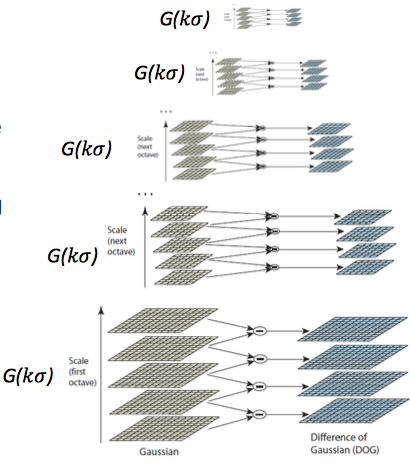
\includegraphics[scale=0.6]{pics/sift}
\caption{Difference of Gaussian. \label{fig:sift}}
\end{center}
\end{figure}
\subsubsection*{Summary}
\begin{itemize}
\item An approach to detect and describe regions of interest in an image.
\item SIFT detector = DoG detector.
\item SIFT features are reasonably invariant to changes in rotation, scaling, and changes in viewpoint (up to 60deg) and illumination.
\item Real time but still \textbf{slow} (10Hz on an i7 laptop).
\end{itemize}
The \textbf{repeatability} can be expressed as
\begin{equation}
\frac{\text{number of correspondences detected}}{\text{number correspondences present}}
\end{equation}
The highest repeatability is obtained when sampling 3 scales per octave.\\
\textbf{Influence of Number of Orientation and NUmber of Sub-Patches}: Single orientation histogram is poor at discriminating, but the results continue to improve up to a 4x4 array of histograms with 8 orientations. 
\begin{itemize}
\item \textbf{Descriptor}: 4x4x8 = 128-element 1D vector.
\item \textbf{Location}: 2D vector.
\item \textbf{Scale} of the patch. 1 scalar value.
\item \textbf{Orientation} (angle of the patch). 1 scalar value.
\end{itemize}
\subsubsection*{SIFT for object recognition}
Can be simply implemented by returning as best object match the one with the largest number of correspondences with the template (object to detect). 4 or 5 point RANSAC can be used to remove outliers.
\subsection*{Feature Matching}
Given a feature $I_1$, how to find the best match in $I_2$?
\begin{enumerate}
\item Define distance function that compares two descriptors ((Z)SSD,SAD,NCC, or Hamming distance for binary descriptors (e.g. Census, BRIEF, BRISK).
\item \textbf{Brute-force matching}:
\begin{itemize}
\item Test all the features in $I_2$.
\item Take the one at min distance.
\end{itemize}
\end{enumerate}
\textbf{Issues with closest descriptor:} Can give good scores to very ambiguous (bad) matches (curse of dimensionality). A better approach would be to compute the ratio of distances between the \textit{first} and \textit{second} match:
\begin{equation}
\frac{d(f_1)}{d(f_2)}<\text{Threshold (usually 0.8)},
\end{equation}
where
\begin{equation}
\begin{split}
d(f_1) &\text{ is the distance of the closest neighbor}\\
d(f_2) &\text{ is the distance of the second closest neighbor}
\end{split}
\end{equation}
\textbf{Explanation for distance ratio}: In SIFT, the nerest neighbor is defined as the keypoint with minimum euclidean distance. However, many features from an image 1 may not have any correct match in image 2 because they arise from background cluttere or were \textit{not detected at all} in the image 1. An effective measure is otained by comparing the distance of the closest \textbf{neighbor} to that of the second closest neighbor. Why? Correct matches need to have the closest neighbor significantly closer than the closest incorrect match, to achieve reliable matching. Moreover, for \textbf{false matches}, there will likely be a number of other false matches within similar distances due to the high dimensionality of the feature space. (aka \textbf{curse of dimensionality}). We can think of the second closest match as providing an estimate of the density of false matches within this portion of the feature space, and at the same time identifying specific instances of feature ambiguity.\\
\textbf{Why 0.8?} 
\begin{itemize}
\item Eliminates 90\% of the false matches,
\item Discards less than 5\% of the correct matches.
\end{itemize}
\subsubsection*{SURF (Speeded Up Robust Features)}
\begin{itemize}
\item Based on ideas similar to SIFT.
\item Approximated computation for detection and descriptor.
\item Results are comparable with SIFT but
\begin{itemize}
\item Faster and
\item Shorter descriptors.
\end{itemize}
\end{itemize}
\subsubsection*{FAST detector (Features from Accelerated Segment Test)}
\begin{itemize}
\item Studies intensity of pixels around candidate pixel $C$.
\item $C$ is FAST corner \textbf{if} a set on $N$ contiguous pixels on circle are
\begin{itemize}
\item all brighter than $intensity(C)+threshold$ or
\item all darker than $intensity(C)+threshold$.
\end{itemize}
\item Typically tests for 9 contiguous pixels in a 16 pixel circumference.
\item \textbf{Very fast detector} (100 Mega pixel/second).
\end{itemize}

\subsubsection*{BRIEF descriptor (Binary Robust Independent Elementary Features)}
\begin{itemize}
\item Goal: high speed.
\item \textbf{Binary} descriptor formation
\begin{itemize}
\item Smooth image,
\item For each detected keypoint (e.g. with FAST) \textbf{sample} 256 intensity pairs ($p_1^i,p_2^i$), $i=1-256$ within a squared patch around keypoint.
\item Create an empty 256-element descriptor.
\item For each i-th pair:
\begin{itemize}
\item if $I_{p_1^i}<I_{p_2^i}$, then set i-th bit of descriptor to 1.
\item else to 0.
\end{itemize}
\end{itemize}
\item The \textbf{pattern is generated randomly} (or by ML) only once: then, same pattern is used for all patches.
\item Pros: \textbf{Binary Descriptor} allows very fast Hamming distance matching: count the number of bits that are different in the descriptors matched.
\item Cons: \textbf{Not scale/rotation invariant}.
\end{itemize}
\subsubsection*{ORB descriptor (Oriented FAST and Rotated BRIEF)}
\begin{itemize}
\item Keypoint detector based on FAST.
\item BRIEF descriptors are steered(?) according to keypoint orientation (to provide rotation invariance).
\item Good binary features are learned by minimizing the correlation on a set of training patches.
\end{itemize}

\subsubsection*{BRISK descriptor (Binary Robust Invariant Scalable Keypoints)}
\begin{itemize}
\item \textbf{Binary}: formed by pairwise intensity comparisons.
\item \textbf{Pattern} defines intensity comparisons in the keypoint neighborhood.
\item \textbf{Red circles}: size of the smoothing kernel applied.
\item \textbf{Blue circles}: smoothed pixel values used.
\item Compare short- and long-distance pairs for orientation assignment and descriptor formation.
\item Detector and descriptor speed: circa \textbf{10 times faster than SURF}.
\item Slower than BRIEF, but scale- and rotation- invariant.
\end{itemize}

\begin{figure}[tbh]
\begin{center}
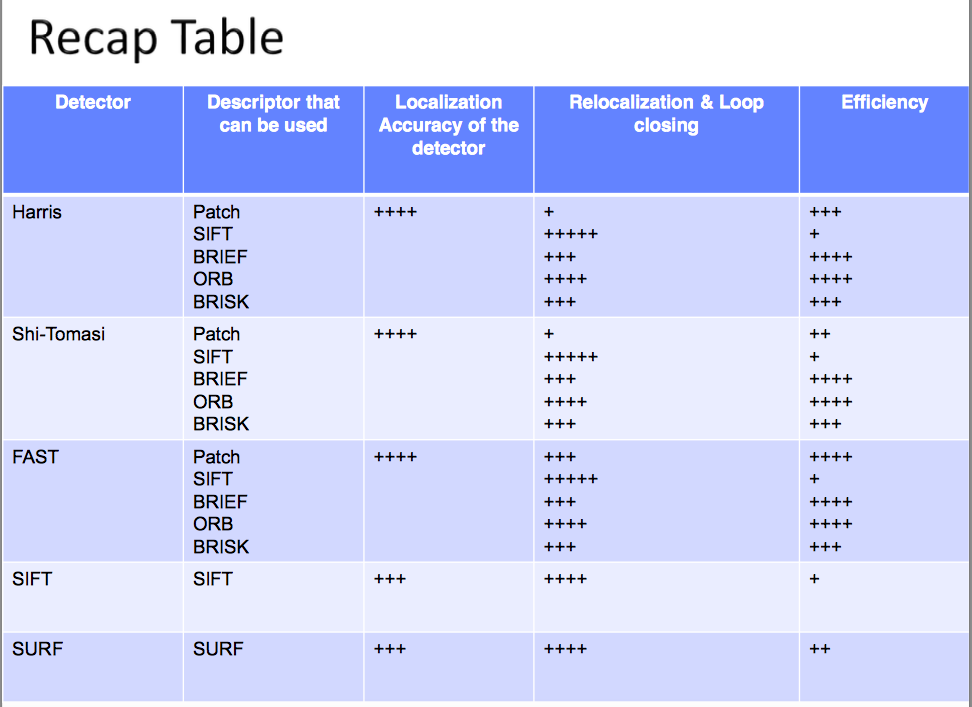
\includegraphics[scale=0.4]{pics/recap}
\caption{Recap for detectors and descriptors. \label{fig:recap}}
\end{center}
\end{figure}
\subsubsection*{Things to remember}
\begin{itemize}
\item Similarity metrics: NCC (ZNCC), SSD (ZSSD), SAD (ZSAD), Census Transform.
\item Point feature detection:
\begin{itemize}
\item Properties and invariance to transformations:
\textbf{Challenges} are rotation, scale, view-point and illumination changes.
\item Extraction:
\begin{itemize}
\item Moravec
\item Harris and Shi-Tomasi: rotation invariance.
\end{itemize}
\item Automatic Scale Detection
\item Descriptor
\begin{itemize}
\item Intensity patches: 
\begin{itemize}
\item Canonical representation: how to make them invariant to transformations: rotation, scale, illumination and view point (affine).
\end{itemize}
\item Better solution: Histogram of oriented gradients: SIFT descriptor.
\end{itemize}
\item Matching:
\begin{itemize}
\item (Z)SSD, SAD, NCC, Hamming distance (last one only for binary descriptors), ration first/second closest descriptor.
\end{itemize}
\item Depending on the task, you may want to trade off repeatability and robustness for speed: approximated solutions, combinations of efficient detectors and descriptors.
\begin{itemize}
\item Fast corner detector,
\item Keypoint descriptors faster than SIFT: SURF, BRIEF, ORB, BRISK.
\end{itemize}
\end{itemize}
\end{itemize}

\newpage
\section*{Lecture 07: Multiple View Geometry 1}
We have different problem statements:
\begin{itemize}
\item \textbf{3D reconstruction from multiple views}
\begin{itemize}
\item \textbf{Assumption:} $K,T,R$ are known.
\item \textbf{Goal:} Recover the 3D structure from images.
\end{itemize}
\item \textbf{Structure from motion}
\begin{itemize}
\item \textbf{Assumption:} $K,T,R$ are unknown.
\item \textbf{Goal:} Recover simultaneously 3D scene structure and camera poses (up to scale) from multiple images.
\end{itemize}
\end{itemize}
For a 2-view geometry, we can define the same problems as
\begin{itemize}
\item \textbf{Depth from stereo (stereo vision)}
\begin{itemize}
\item \textbf{Assumption:} $K,T,R$ are known.
\item \textbf{Goal:} Recover the 3D structure from images.
\end{itemize}
\item \textbf{2-view structure from motion}
\begin{itemize}
\item \textbf{Assumption:} $K,T,R$ are unknown.
\item \textbf{Goal:} Recover simultaneously 3D scene structure and camera poses (up to scale) and intrinsic parameters from two different views of the scene.
\end{itemize}
\end{itemize}
\subsection*{Depth from stereo}
From a single camera, we can only compute the \textbf{ray} on which each image point lies. With a stereo camera (binocular), we can solve for the intersection of the rays and eventually recover the 3D structure.
\subsubsection*{The human binocular system}
\textbf{Stereopsys:} the brain allows us to see the left and right retinal images as a single 3D image. The images project on our retina up-side-down but our brains let us perceive them as straight. Radial distortion is removed. This process is also known as \textbf{rectification}. The distance of two seen images is called \textbf{disparity} (allows us to perceive the depth). An application of this concept are \textbf{stereograms}.
\subsubsection*{Stereo Vision: basics}
The basic principle behind stereo vision is \textbf{triangulation}.
\begin{itemize}
\item Gives reconstruction as intersection of two rays.
\item Requires \textbf{camera pose (calibration) and point correspondence}.
\end{itemize}
There are basically two cases
\begin{enumerate}
\item Simplified case: identical cameras are \textbf{aligned}. 
\item General case: different cameras are not \textbf{aligned}.
\end{enumerate}
\subsubsection*{Simplified Case}
\begin{figure}[tbh]
\begin{center}
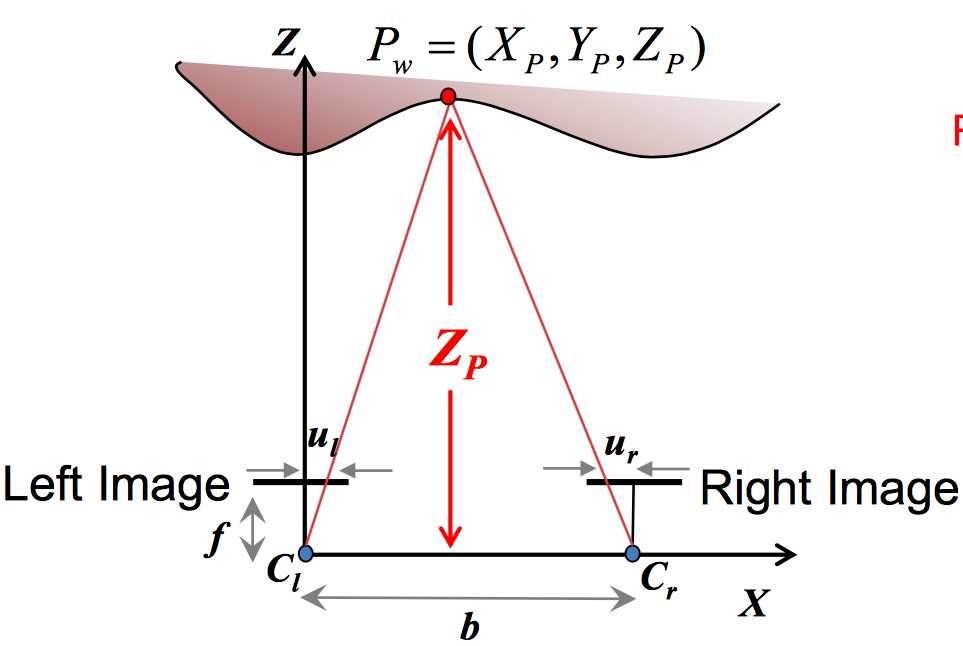
\includegraphics[scale=0.3]{pics/stereo_vis}
\caption{Simplified case for stereo vision. \label{fig:stereo_vis}}
\end{center}
\end{figure}
The two cameras are identical, meaning that they have the same \textbf{focal length}, and are \textbf{aligned} with the $x$-axis. If we have a world point $P_w$, a distance from the axis to the point $Z_P$, a distance between the cameras $b$ and focal length $f$, we can use similar triangles from Figure \ref{fig:stereo_vis} and get
\begin{equation}
\begin{split}
\frac{f}{Z_P}&=\frac{u_l}{X_P}\\
\frac{f}{Z_P}&=\frac{-u_r}{b-X_P}\\
\Rightarrow Z_P&=\frac{b\cdot f}{u_l-u_r}.
\end{split}
\end{equation}
The difference $u_l-u_r$ is called \textbf{disparity}: difference in image location of the projection of a 3D point on two image planes. (QUESTIONS)\\
What is the optimal baseline?
\begin{itemize}
\item \textbf{Too small:}
\begin{itemize}
\item Large depth error
\end{itemize}
\item \textbf{Too large:}
\begin{itemize}
\item Minimum measurable distance increases.
\item Difficult search problem for close objects.
\end{itemize}
\end{itemize}
\subsubsection*{General Case: triangulation}
In reality no cameras are identical and aligning both cameras on a horizontal axis is impossible. (WHY?). In order to be able to use a stereo camera, we need to compute
\begin{itemize}
\item The extrinsic parameters (relative rotation and translation)
\item the intrinsic parameters (focal length, optical center, radial distortion of each camera).
\end{itemize}
In order to do this we use calibration methods (Tsai or homographies). How do we get the \textbf{relative pose?} Lines do not always interset in the 3D space: we want to minimize the error. For the two cameras we have
\begin{equation}
\tilde{p}_l=\lambda_l\cdot \begin{pmatrix}
 u_l\\
 v_l\\
 1
 \end{pmatrix}=K_l\cdot \begin{pmatrix}
 X_w\\
 Y_w\\
 Z_w
 \end{pmatrix}, \quad \tilde{p}_r=\lambda_r\cdot \begin{pmatrix}
 u_r\\
 v_r\\
 1
 \end{pmatrix}=K_r\cdot R\cdot \begin{pmatrix}
 X_w\\
 Y_w\\
 Z_w
 \end{pmatrix}+T. 
\end{equation}
In order to triangulate, we use \textbf{least-squares} approximation:
\begin{equation}
\begin{split}
\lambda_1\cdot \begin{pmatrix}
 u_1\\
 v_1\\
 1
 \end{pmatrix}=K\cdot [I|0]\cdot \begin{pmatrix}
 X_w\\
 Y_w\\
 Z_w\\
 1
 \end{pmatrix}&\Rightarrow \lambda_1p_1=M_1\cdot P \qquad \text{left camera}. \\
 \lambda_2\cdot \begin{pmatrix}
 u_2\\
 v_2\\
 1
 \end{pmatrix}=K\cdot [R|T]\cdot \begin{pmatrix}
 X_w\\
 Y_w\\
 Z_w\\
 1
 \end{pmatrix}&\Rightarrow \lambda_2p_2=M_2\cdot P \qquad \text{right camera}.
\end{split}
\end{equation}
We solve for $P$ and get a system $A\cdot \begin{pmatrix} \lambda_1 \\\lambda_2 \end{pmatrix}=b$, which cannot be inverted (A is $3\times 2$). We use pseudoinverse approximation (least squares) and get
\begin{equation}
A^T\cdot A\cdot \begin{pmatrix}
 \lambda_1\\
 \lambda_2
 \end{pmatrix}=A^T\cdot b \Rightarrow \begin{pmatrix}
 \lambda_1\\
 \lambda_2
 \end{pmatrix}=(A^T\cdot A)^{-1}\cdot A^T\cdot b
\end{equation}
\textbf{Interpretation:} Given the projections $p_{1,2}$ of a 3D point $P$ in two or more images, we want to find the coordinates of the 3D point by intersecting the two rays corresponding to the projections. We want to find the shortest segment connecting the two viewing rays and let $P$ be the \textbf{midpoint} of the segment.
\subsubsection*{Triangulation: nonlinear approach}
We want to find $P$ that minimizes the \textbf{sum of squared reprojection error}
\begin{equation}
SSRE=d^2(p_1,\pi_1(P))+d^2(p_2,\pi_2(P)),
\end{equation}
where 
\begin{equation}
d(p_1,\pi_1(P))=||p_1-\pi_1(P)||
\end{equation}
is called \textbf{reprojection error}. In practice, this is done by initializing $P$ using linear approach and then minimize SSRE using Gauss-Newton of Levenberg-Marquardt.
\subsubsection*{Correspondence Problem}
Given a point $p$ in a first image, where is its corresponding point $p'$ in the right image? \\
\textbf{Correspondence Search}: Identify image patches in the left and in the right images, corresponding to the same scene structure. Similarity measures:
\begin{itemize}
\item (Z)ZNCC
\item (Z)SSD
\item (Z)SAD
\item Census Transform
\end{itemize}
\textbf{Problem:} Exhaustive image search can be computationally very expensive! Can we do that in 1D?\\
$\rightarrow$ potential matches for $p$ have to lie on the corresponding epipolar line $l'$.
\begin{itemize}
\item The \textbf{epipolar line} is the projection of the infinite ray $\pi^{-1}(p)$ corresponding to $p$ in the other camera image.
\item The \textbf{epipole} is the projection of the optical center on the other camera image.
\item A \textbf{stereo camera} has two epipoles!
\end{itemize}
\begin{figure}[tbh]
\begin{center}
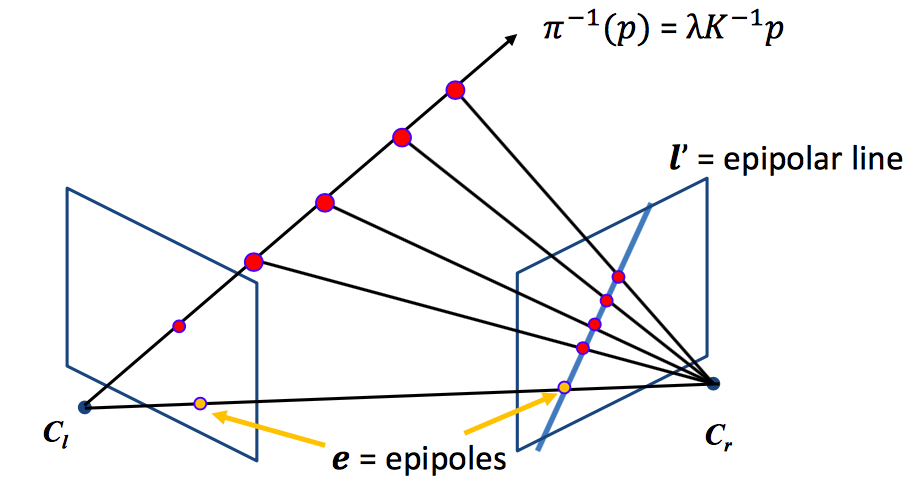
\includegraphics[scale=0.4]{pics/epi}
\caption{Epipolar lines and epipoles. \label{fig:epi}}
\end{center}
\end{figure}
\subsubsection*{The Epipolar Constraint}
\begin{itemize}
\item The epipolar plane is uniquely defined by the two optical centers $C_l,C_r$ and one image point $p$. 
\item The \textbf{epipolar constraint} constraints the location, in the second view, of the corresponding point to a given point in the first view.
\item $\Rightarrow$ This reduces the search to 1D problem along conjugate epipolar lines.
\end{itemize}
\subsubsection*{Example: converging cameras}
\textbf{Important:} All epipolar lines intersect at the epipole! As the position od the 3D point varies, the epipolar line \textit{rotates} about the baseline. 
\subsubsection*{Example: forward motion}
Epipoles have the same coordinates in both images: points move along lines radiating from $e$: \textit{Focus of expansion}
\subsubsection*{Stereo Rectification}
\begin{itemize}
\item Even in commercial stereo cameras, left and right images are not aligned.
\item It is convenient if image scanlines are the epipolar lines
\item Stereo rectification warps left and right images into new \textit{rectified} images, whose epipolar lines are algined to the baseline.
\end{itemize}
\begin{figure}[tbh]
\begin{center}
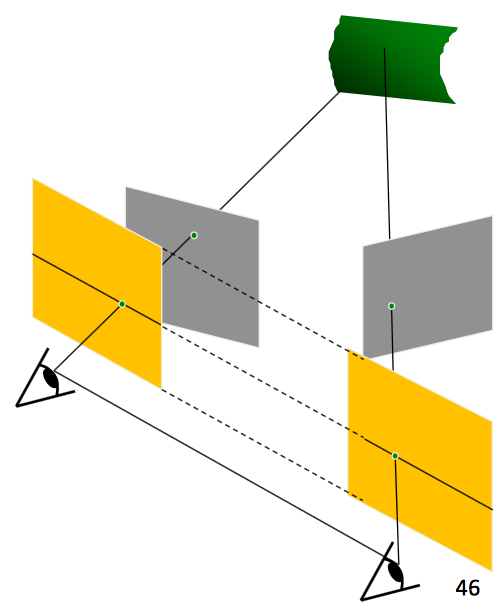
\includegraphics[scale=0.3]{pics/rectif}
\caption{Stereo Rectification. \label{fig:rectif}}
\end{center}
\end{figure}
\begin{itemize}
\item Reprojects image planes onto a common plane parallel to the baseline.
\item It works by computing two homographies, one for each input image reprojection.
\item $\Rightarrow$ Then, scanlines are \textbf{aligned} and epipolar lines are \textbf{horizontal}.
\end{itemize}
\textbf{Idea:} we define two new Perspective Projection Matrices obtained by rotating the old ones around their optical centers, until focal planes become coplanar (containing the baseline). This ensures \textbf{epipoles at infinity}. In order to have horizontal epipolar lines, the baseline should be \textit{parallel} to the new X axis of both cameras. Moreover, corresponding points should have \textbf{the same vertical coordinate}. This is obtained by having same intrinsic parameters for the new cameras. Since the the focal length is the same, the new image planes are coplanar. PPMs are the same as the old cameras, whereas the new orientation (the same for both cameras) differs from the old ones by suitable rotations. For both cameras, \textbf{intrinsic parameters are the same}.
\subsubsection*{Implementation}
\begin{enumerate}
\item The perspective equation for a point in the world is 
\begin{equation}
\text{image point}=\tilde{p}=\begin{pmatrix}
\tilde{u}\\
\tilde{v}\\
\tilde{w}
\end{pmatrix} = \lambda \begin{pmatrix}
 u\\
 v\\
 1
 \end{pmatrix}=K[R|T]\cdot \begin{pmatrix}
 X_w\\
 Y_w\\
 Z_w\\
 1
 \end{pmatrix}.
 \end{equation}
This can be rewritten in a more convenient way by considering $[R|T]$ as the transformation from the world to the Camera frame ($T$ expressed as $C$):
\begin{equation}
 \lambda \begin{pmatrix}
 u\\
 v\\
 1
 \end{pmatrix}=K\cdot R^{-1}\cdot \left(\begin{pmatrix}
 X_w\\
 Y_w\\
 Z_w
 \end{pmatrix}-C\right)
\end{equation}
\item We can then write the Perspective Equation for the Left and Right cameras: we assume for generality that they have the same intrinsic parameters:
\begin{equation}
\begin{split}
\lambda_L\cdot \begin{pmatrix}
 u_L\\
 v_L\\
 1
 \end{pmatrix}&= K_L\cdot R_L^{-1}\cdot \left(\begin{pmatrix}
 X_w\\
 Y_w\\
 Z_w
 \end{pmatrix}-C_L\right) \quad \text{left camera}\\
 \lambda_R\cdot \begin{pmatrix}
 u_R\\
 v_R\\
 1
 \end{pmatrix}&= K_R\cdot R_R^{-1}\cdot \left(\begin{pmatrix}
 X_w\\
 Y_w\\
 Z_w
 \end{pmatrix}-C_R\right) \quad \text{right camera}
\end{split}
\end{equation}
\item The goal of stereo rectification is to warp left and right camera images such that their focal planes are coplanar and the intrinsic parameters are identical. It follows 
\begin{equation}
\begin{split}
\lambda_L\cdot \begin{pmatrix}
 u_L\\
 v_L\\
 1
 \end{pmatrix}&= K_L\cdot R_L^{-1}\cdot \left(\begin{pmatrix}
 X_w\\
 Y_w\\
 Z_w
 \end{pmatrix}-C_L\right) \rightarrow \overline{\lambda}_L\cdot \begin{pmatrix}
 \overline{u}_L\\
 \overline{v}_L\\
 1
 \end{pmatrix}= \overline{K}\cdot \overline{R}^{-1}\cdot \left(\begin{pmatrix}
 X_w\\
 Y_w\\
 Z_w
 \end{pmatrix}-C_L\right) \\
 \lambda_R\cdot \begin{pmatrix}
 u_R\\
 v_R\\
 1
 \end{pmatrix}&= K_R\cdot R_R^{-1}\cdot \left(\begin{pmatrix}
 X_w\\
 Y_w\\
 Z_w
 \end{pmatrix}-C_R\right) \rightarrow \overline{\lambda}_R\cdot \begin{pmatrix}
 \overline{u}_R\\
 \overline{v}_R\\
 1
 \end{pmatrix}= \overline{K}\cdot \overline{R}^{-1}\cdot \left(\begin{pmatrix}
 X_w\\
 Y_w\\
 Z_w
 \end{pmatrix}-C_R\right) 
\end{split}
\end{equation}
\item By solving for $\begin{pmatrix}
 X_w\\
 Y_w\\
 Z_w \end{pmatrix}$ for each camera, we can compute the Homography (or warping) that needs to be applied to rectify each camera image:
\begin{equation}
\begin{split}
\overline{\lambda}_L\cdot \begin{pmatrix}
 \overline{u}_L\\
 \overline{v}_L\\
 1
 \end{pmatrix}&=\lambda_L \cdot \underbrace{\overline{K}\cdot \overline{R}^{-1} \cdot R_L \cdot K_L^{-1}}_{\text{homography left camera}} \cdot \begin{pmatrix}
 u_L\\
 v_L\\
 1
 \end{pmatrix}\\
 \overline{\lambda}_R\cdot \begin{pmatrix}
 \overline{u}_R\\
 \overline{v}_R\\
 1
 \end{pmatrix}&=\lambda_R \cdot \underbrace{\overline{K}\cdot \overline{R}^{-1} \cdot R_R \cdot K_R^{-1}}_{\text{homography right camera}} \cdot \begin{pmatrix}
 u_R\\
 v_R\\
 1
 \end{pmatrix}
\end{split}
\end{equation}
\item The new $\overline{K},\overline{R}$ can be chosen as
\begin{equation}
\begin{split}
\overline{K}&=\frac{K_L+K_R}{2}\\
\overline{R}&=[\overline{r}_1,\overline{r}_2,\overline{r}_3],
\end{split}
\end{equation}
where $\overline{r}_1,\overline{r}_2,\overline{r}_3$ are the column vectors of $\overline{R}$. These can be computed as
\begin{equation}
\begin{split}
\overline{r}_1&=\frac{C_2-C_1}{||C_2-C_1||}\\
\overline{r}_2&=r_3 \times \overline{r_1} \text{ where }r_3 \text{is the third column of }R_L\\
\overline{r}_3&=\overline{r}_1\times \overline{r}_2.
\end{split}
\end{equation}
For more details have a look at \textit{A compact alg. for rectification of stereo pairs}.
\end{enumerate}
\textbf{Example:} First, you remove the radial distotion (use e.g. bilinear interpolation). Then, compute homographies and rectify (bilinear interpolation). \\
In order to solve the correspondence problem, one can use a window around the point of interest and use similarity measures to find neighborhoods.
\subsubsection*{Correlation-based window matching}
\begin{itemize}
\item Problem: textureless regions (\textbf{aperture problem}), high ambiguity! \textbf{Solution:} increase window size to distinguish!
\begin{itemize}
\item Smaller window: \textbf{more detail but more noise}!
\item Larger window: \textbf{smoother disparity maps but less detail}
\end{itemize}
\end{itemize}
\subsubsection*{Disparity Map}
Input to dense 3D reconstruction
\begin{enumerate}
\item For each pixel in the left image, find its corresponding point in the right image.
\item Compute the disparity for each pair of correspondences.
\item Visualized in gray-scale or color coded image.
\end{enumerate}
The depth $Z$ can be computed from the disparity by recalling that
\begin{equation}
Z_P=\frac{bf}{u_l-u_r}
\end{equation}
Challenges include: occlusion, repetition, non-lambertian surfaces (specularities), textureless surfaces.
\subsubsection*{Improvements:}
Multiple match could satisfy the epipolar constraint. A good way to address the problem would be to have
\begin{itemize}
\item Uniqueness: only one match in right image for every point in left image.
\item Ordering: points on same surface will be in same order in both views
\item Disparity gradient: disparity changes smoothly between points on the same surface.
\end{itemize}
\textbf{Sparse Stereo Correspondence} restrict search to sparse set.
\newpage
\section*{Lecture 08 - Multiple View Geometry 2}
\subsection*{Two-view Structure from Motion}
\textbf{Problem formulation:} Given $n$ point correspondences between two images, $\{p_1^i=(u_1^i,v_1^i), \ p_2^i=(u_2^i,v_2^i)\}$, simultaneously estimate the 3D points $P^i$, the camera relative-motion parameters ($R,T$), and the camera intrinsics $K_1,K_2$ that satisfy:
\begin{equation}
\begin{split}
\lambda_1 \cdot \begin{pmatrix}
 u_1^i\\
 v_1^i\\
 1
 \end{pmatrix}&=K_1\cdot [I|0]\cdot \begin{pmatrix}
 X_w^i\\
 Y_w^i\\
 Z_w^i\\
 1
 \end{pmatrix},\\
 \lambda_2 \cdot \begin{pmatrix}
 u_2^i\\
 v_2^i\\
 1
 \end{pmatrix}&=K_2\cdot [R|T]\cdot \begin{pmatrix}
 X_w^i\\
 Y_w^i\\
 Z_w^i\\
 1
 \end{pmatrix}
\end{split}
\end{equation}
We have two cases then:
\subsubsection*{Calibrated Cameras ($K_1,K_2$ known)}
For convenience, we use \textit{normalized image coordinates}
\begin{equation}
\begin{pmatrix}
\bar{u}\\
\bar{v}\\
1
\end{pmatrix}=K^{-1}\cdot \begin{pmatrix}
u\\
v\\
1
\end{pmatrix}.
\end{equation}
We want to find $R,T,P^i$ which satisfy
\begin{equation}
\begin{split}
\lambda_1 \cdot \begin{pmatrix}
 \bar{u}_1^i\\
 \bar{v}_1^i\\
 1
 \end{pmatrix}&=K_1\cdot [I|0]\cdot \begin{pmatrix}
 X_w^i\\
 Y_w^i\\
 Z_w^i\\
 1
 \end{pmatrix},\\
 \lambda_2 \cdot \begin{pmatrix}
 \bar{u}_2^i\\
 \bar{v}_2^i\\
 1
 \end{pmatrix}&=K_2\cdot [R|T]\cdot \begin{pmatrix}
 X_w^i\\
 Y_w^i\\
 Z_w^i\\
 1
 \end{pmatrix}.
\end{split}
\end{equation}
\textbf{Scale Ambiguity}: If we rescale the entire scene by a constant factor (i.e. similarity transformation), the projections (in pixels) of the scene points in both images remain the \textbf{same}.
\begin{itemize}
\item In \textit{monocular} vision it is \textbf{not possible} to recover the absolute scale of the scene.
\item In \textit{stereo vision}, only \textbf{5 degrees of freedom} are measurable:
\begin{itemize}
\item 3 parameters to describe the \textbf{rotation}.
\item 2 parameters for the \textbf{translation up to a scale} (we can only compute the direction of translation but not its length (magnitude)).
\end{itemize}
\end{itemize}
How many knowns and unknowns?
\begin{itemize}
\item $4n$ knowns: $n$ correspondences, each one $(u_1^i,v_1^i)$ and $(u_2^i,v_2^i)$, $i=1,\hdots,n$.
\item $5+3n$ unknowns: 5 for the motion up to a scale (3 rotation and 2 translation) and $3n$ which is the number of coordinates of the $n$ 3D points.
\end{itemize}
It should hold
\begin{equation}
\begin{split}
4n &\geq 5+3n\\
\Rightarrow n&\geq 5.
\end{split}
\end{equation}
The first analytical solution for 5 points was given by Kruppa in 1913 (10 degree order polynomial, up to 10 solution with complex ones).\\
Let's define the \textbf{cross product} as a matrix multiplication
\begin{equation}
a\times b = \begin{pmatrix}
 0&-a_z&a_y\\
 a_z&0&-a_x\\
 -a_y&a_x&0
 \end{pmatrix}\cdot \begin{pmatrix}
 b_x\\
 b_y\\
 b_z
 \end{pmatrix}=[a]_x\cdot b
\end{equation}
\subsubsection*{Epipolar Geometry}
\begin{equation}
\bar{p}_1=\begin{pmatrix}
\bar{u}_1\\
\bar{v}_1\\
1
\end{pmatrix},\quad \bar{p}_2=\begin{pmatrix}
\bar{u}_2\\
\bar{v}_2\\
1
\end{pmatrix}
\end{equation}
We can observe that $p_1,p_2,T$ are coplanar:
\begin{equation}
\begin{split}
p_2^T\cdot n&=0\\
p_2^T\cdot (T\times p_1')&=0\\
p_2^T \cdot (T\times (Rp_1))&=0\\
p_2^T\cdot [T]_x\cdot Rp_1&=0\\
p_2^T \cdot E \cdot p_1&=0 \text{ is the epipolar constraint, where }E=[T]_x\cdot R \text{ is the essential matrix}.
\end{split}
\end{equation}
Applying the constraints results in \textit{four different} solutions for $R$ and $T$.
\begin{figure}[h!]
\begin{center}
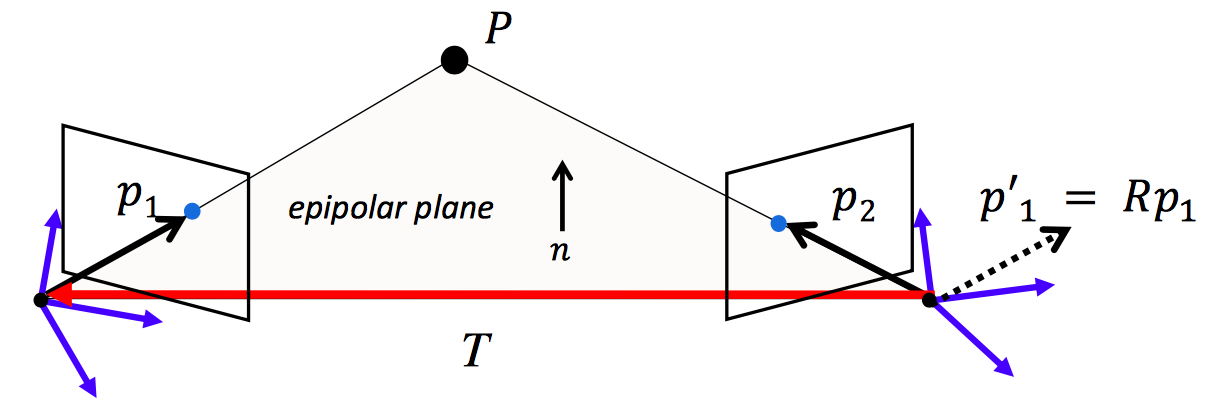
\includegraphics[scale=0.3]{pics/epi_2}
\caption{Epipolar constraint \label{fig:epi_2}}
\end{center}
\end{figure}
\subsubsection*{How to compute the Essential Matrix}
Kruppa's solution is not efficient. In 1996, Philipp proposed an iterative solution. In 2004, the first efficient non iterative solution was proposed. This uses \textbf{Groebner Decomposition}. The first popular solution uses 8 points and is called the \textbf{8 point algorithm or Longuet-Higgins algorithm} (still used in NASA rovers).
\subsubsection*{The 8-point Algorithm}
The Essential matrix is defined by
\begin{equation}
\bar{p}_2^T\cdot E \bar{p}_1=0.
\end{equation}
Each pair of point correspondences provides a linear equation. For $n$ points we can write
\begin{equation}
\underbrace{\begin{pmatrix}
\bar{u}_2^1\cdot \bar{u}_1^1&\bar{u}_2^1\cdot \bar{v}_1^1&\bar{u}_2^1&\bar{v}_2^1\cdot \bar{u}_1^1&\bar{v}_2^1\cdot \bar{v}_1^1&\bar{v}_2^1&\bar{u}_1^1&\bar{v}_1^1&1\\
\bar{u}_2^2\cdot \bar{u}_1^2&\bar{u}_2^2\cdot \bar{v}_1^2&\bar{u}_2^2&\bar{v}_2^2\cdot \bar{u}_1^2&\bar{v}_2^2\cdot \bar{v}_1^2&\bar{v}_2^2&\bar{u}_1^2&\bar{v}_1^2&1\\
\vdots &\vdots &\vdots &\vdots &\vdots &\vdots &\vdots &\vdots &\vdots \\
\bar{u}_2^n\cdot \bar{u}_1^n&\bar{u}_2^n\cdot \bar{v}_1^n&\bar{u}_2^n&\bar{v}_2^n\cdot \bar{u}_1^n&\bar{v}_2^n\cdot \bar{v}_1^n&\bar{v}_2^n&\bar{u}_1^n&\bar{v}_1^n&1
\end{pmatrix}}_{Q \text{ (known) }}\cdot  \underbrace{\begin{pmatrix}
e_{11}\\
e_{12}\\
e_{13}\\
e_{21}\\
e_{22}\\
e_{23}\\
e_{31}\\
e_{32}\\
e_{33}\\
 \end{pmatrix}}_{\bar{E} \text{ unknown }}=0
\end{equation}
This problem can be written as
\begin{equation}
Q\cdot \bar{E}=0.
\end{equation}
Two types of solution
\begin{itemize}
\item \textbf{Minimal Solution}
\begin{itemize}
\item $Q_{n\times 9}$ should have rank $8$ to have unique (up to scale) non trivial solution $\bar{E}$.
\item Each point correspondence provides 1 independent equation.
\item Thus, 8 point correspondences are needed.
\end{itemize}
\item \textbf{Over-determined Solution}
\begin{itemize}
\item $n>8$ points.
\item A solution is to minimize $||Q\cdot \bar{E}||^2$ subject to the constraint $||\bar{E}||^2=1$. The solution is the eigenvector corresponding to the smallest eigenvalue of matrix $Q^T\cdot Q$.
\item This can be solved with Singular Value Decomposition.
\end{itemize}
\item \textbf{Degenerate Solution} if 3D points are coplanar. There is the 5 point algorithm which holds also for coplanar points.
\end{itemize}
\subsubsection*{Interpretation}
With the algorithm we try to minimize the \textbf{algebraic error}
\begin{equation}
\sum_{i=1}^{N} (\bar{p}_{2}^{i^T}\cdot E \cdot \bar{p}_1^i)^2,
\end{equation}
where
\begin{equation}
\bar{p}_2^T\cdot E \cdot \bar{p}_1 = ||\bar{p}_2||\cdot ||E\cdot \bar{p}_1||\cdot \cos(\theta)
\end{equation}
which is not zero is $p_1,p_2,T$ are not coplanar.
When extracting solutions, four results are available. We look only at results with points \textbf{in front of both cameras}.
\subsubsection*{Uncalibrated Cameras ($K_1,K_2$ unknown)}
It holds 
\begin{equation}
\bar{p}_2^T\cdot E \bar{p}_1=0,
\end{equation}
where 
\begin{equation}
\begin{pmatrix}
\bar{u}_1^i\\
\bar{v}_1^i\\
1
\end{pmatrix}=K_1^{-1}\cdot \begin{pmatrix}
u_1^i\\
v_1^i\\
1
\end{pmatrix},\quad \begin{pmatrix}
\bar{u}_2^i\\
\bar{v}_2^i\\
1
\end{pmatrix}=K_2^{-1}\cdot \begin{pmatrix}
u_2^i\\
v_2^i\\
1
\end{pmatrix}.
\end{equation}
By rewriting the constraint, one obtains
\begin{equation}
\begin{split}
\begin{pmatrix}
u_2^i\\
v_2^i\\
1
\end{pmatrix}^T\cdot K_2^{-T}\cdot E \cdot K_1^{-1}\cdot \begin{pmatrix}
u_1^i\\
v_1^i\\
1
\end{pmatrix}&=0\\
\begin{pmatrix}
u_2^i\\
v_2^i\\
1
\end{pmatrix}^{T}\cdot F \cdot \begin{pmatrix}
u_1^i\\
v_1^i\\
1
\end{pmatrix}&=0,
\end{split}
\end{equation}
where $F$ is the \textbf{fundamental matrix}, which can be computed as
\begin{equation}
F=K_2^{-T}\cdot E \cdot K_1^{-1}=K_2^{-T}\cdot [T]_x\cdot R \cdot K_1^{-1}.
\end{equation}
The same 8-point algorithm can be used to compute the fundamental matrix:
\begin{equation}
\underbrace{\begin{pmatrix}
\bar{u}_2^1\cdot \bar{u}_1^1&\bar{u}_2^1\cdot \bar{v}_1^1&\bar{u}_2^1&\bar{v}_2^1\cdot \bar{u}_1^1&\bar{v}_2^1\cdot \bar{v}_1^1&\bar{v}_2^1&\bar{u}_1^1&\bar{v}_1^1&1\\
\bar{u}_2^2\cdot \bar{u}_1^2&\bar{u}_2^2\cdot \bar{v}_1^2&\bar{u}_2^2&\bar{v}_2^2\cdot \bar{u}_1^2&\bar{v}_2^2\cdot \bar{v}_1^2&\bar{v}_2^2&\bar{u}_1^2&\bar{v}_1^2&1\\
\vdots &\vdots &\vdots &\vdots &\vdots &\vdots &\vdots &\vdots &\vdots \\
\bar{u}_2^n\cdot \bar{u}_1^n&\bar{u}_2^n\cdot \bar{v}_1^n&\bar{u}_2^n&\bar{v}_2^n\cdot \bar{u}_1^n&\bar{v}_2^n\cdot \bar{v}_1^n&\bar{v}_2^n&\bar{u}_1^n&\bar{v}_1^n&1
\end{pmatrix}}_{Q \text{ (known) }}\cdot  \underbrace{\begin{pmatrix}
f_{11}\\
f_{12}\\
f_{13}\\
f_{21}\\
f_{22}\\
f_{23}\\
f_{31}\\
f_{32}\\
f_{33}\\
 \end{pmatrix}}_{\bar{F} \text{ unknown }}=0
\end{equation}
There are \textbf{orders of magnitude} of difference, which leads to poor results with least-squares. How to solve?
\subsubsection*{Normalized 8-point algorithm}
This estimates the Fundamental matrix on a set of \textbf{Normalized correspondences} (with better numerical properties) and then \textbf{unnormalizes} the result to obtain the fundamental matrix for the original given correspondences. \\
\textbf{Idea:} Transform image coordinates so that they are in the range $[-1,1]\times [-1,1]$. One way is to apply the following rescaling and shift
\begin{figure}[h!]
\begin{center}
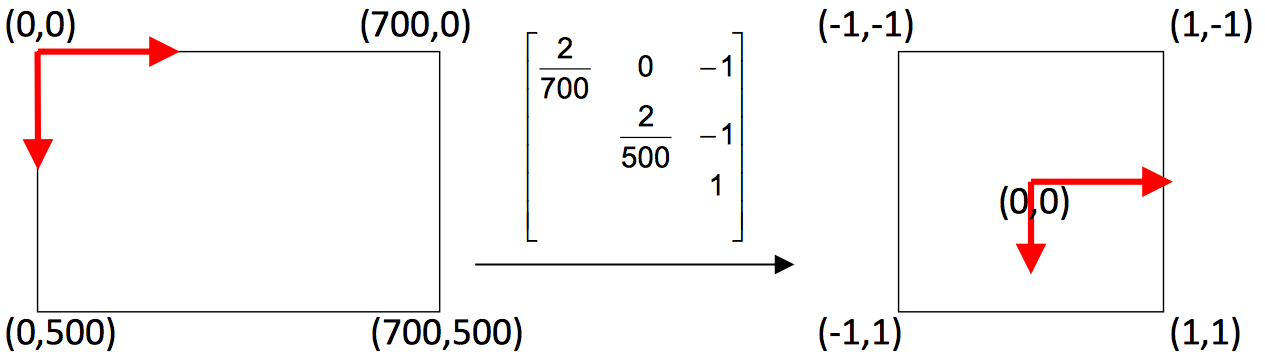
\includegraphics[scale=0.3]{pics/shift}
\caption{Shift for normalized algorithm. \label{fig:shift}}
\end{center}
\end{figure}
A more popular is to rescale the two point sets such that the centroid of each is 0 and the mean standard deviation $\sqrt{2}$. This can be done for every point as follows
\begin{equation}
\hat{p}^i=\frac{\sqrt{2}}{\sigma}\cdot (p^i-\mu),
\end{equation}
where
\begin{equation}
\mu=\frac{1}{N}\sum_{i=1}^n p^i
\end{equation}
is the centroid of the set and $\sigma=\frac{1}{N}\sum_{i=1}^n ||p^i-\mu||^2$ is the mean standard deviation. This transformation can be expressed in matrix form
\begin{equation}
\hat{p}^i=\begin{pmatrix}
\frac{\sqrt{2}}{\sigma}&0&-\frac{\sqrt{2}}{\sigma}\mu^x\\
0&\frac{\sqrt{2}}{\sigma}&-\frac{\sqrt{2}}{\sigma}\mu^y\\
0&0&1
\end{pmatrix}\cdot p^i.
\end{equation}
The algoritm at the end reads
\begin{enumerate}
\item Normalize point correspondences: $\hat{p}_1=B_1\cdot p_1$, $\hat{p}_2=B_2\cdot p_2$.
\item Estimate $\hat{F}$ using normalized coordinates $\hat{p}_1,\hat{p}_2$.
\item Compute $F$ from $\hat{F}:$
\begin{equation}
\begin{split}
\hat{p}_2^T\cdot \hat{F}\cdot \hat{p}_1&=0\\
B_2^T\cdot p_2^{T}\cdot \hat{F}\cdot \cdot B_1^T\cdot p_1^T&=0\\
\Rightarrow F&=B_2^T\cdot \hat{F}\cdot B_1
\end{split}
\end{equation}
\end{enumerate}
\subsubsection*{Error Measures}
The quality of the estimated fundamental matrix can be measured by looking at cost functions. The first is defined using the Epipolar Constraint
\begin{equation}
err = \sum_{i=1}^{N}(\bar{p}_2^{i^T}\cdot E \cdot p_1^{i})^2
\end{equation}
This error will exactly be 0 if computed from 8 points. For more points not 0 because of image noise/outliers. Better methods are
\subsubsection*{Directional Error}
Sum of the angular distances to the Epipolar plane: $err=\sum_i (\cos(\theta_i))^2$, where
\begin{equation}
cos(\theta)=\left(\frac{p_2^T\cdot E \cdot p_1}{||p_2^T||\cdot ||E\cdot p_1||} \right)
\end{equation}
\subsubsection*{Epipolar Line Distance}
\textbf{Squared Epipolar-Line-to-point Distances}
\begin{equation}
err=\sum_{i=1}^Nd^2(p_1^i,l_1^i)+d^2(p_2^i,l_2^i).
\end{equation}
Cheaper than reprojection error: does not require point triangulation!
\begin{figure}[h!]
\begin{center}
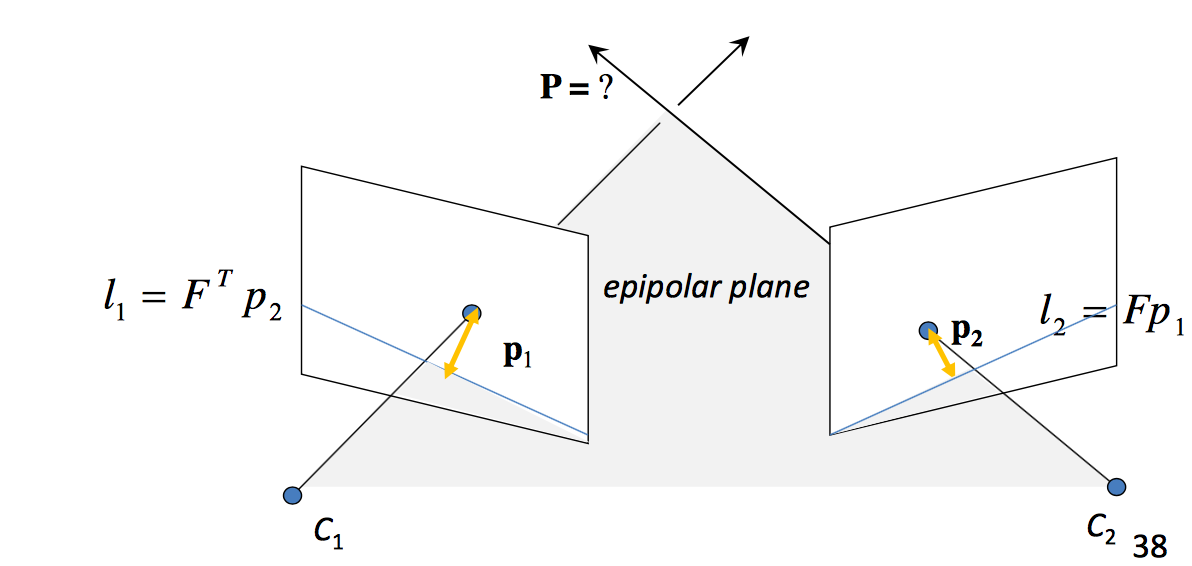
\includegraphics[scale=0.3]{pics/epi_line}
\caption{Epipolar Line Distance. \label{fig:epi_line}}
\end{center}
\end{figure}
\subsubsection*{Reprojection Error}
Sum of the \textbf{Squared Reprojection Errors}
\begin{equation}
err=\sum_{i=1}^N ||p_1^i-\pi_1(P^i)||^2+||p_2^i-\pi_2(P^i,R,T)||^2
\end{equation}
Computation is expensive because of point triangulation, but is the \textbf{most accurate}!
\begin{figure}[h!]
\begin{center}
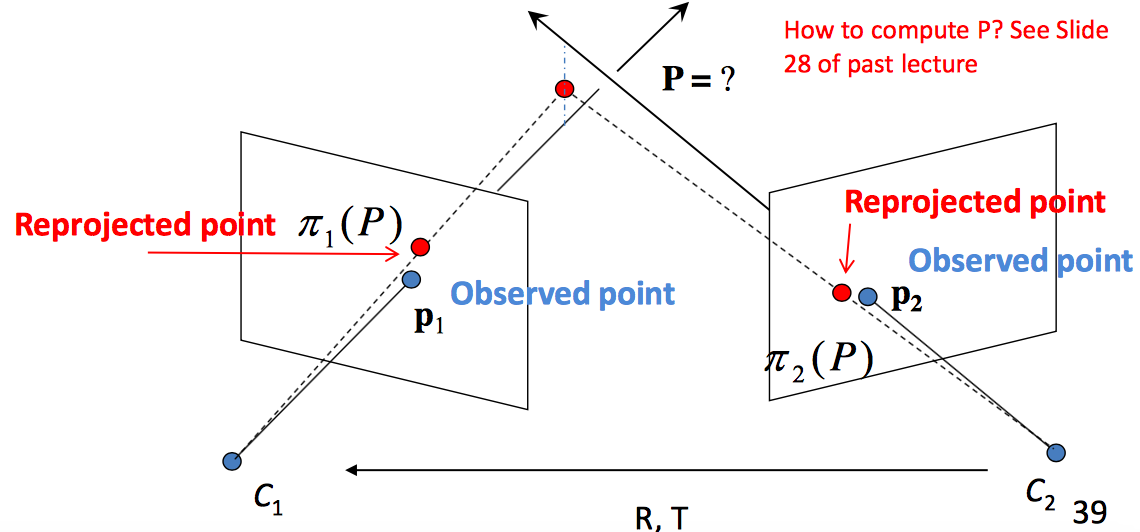
\includegraphics[scale=0.3]{pics/repro}
\caption{Reprojection Error. \label{fig:repro}}
\end{center}
\end{figure}
\subsection*{Robust Structure From Motion}
Matched points are usually contaminated by \textbf{outliers}. Causes for this are
\begin{itemize}
\item Change in view point
\item Image noise
\item Occlusions
\item Blur
\end{itemize}
The task of removing them is for \textbf{Robust Estimation}. Since error is integrating over time, this increases and is really bad.
\subsubsection*{RANSAC (Random Sample Consensus)}
Ransac is the standard method for \textbf{model fitting in the presence of outliers} (noise points or wrong data). It can be applied to all problems where the goal is to estimate parameters of a model from the data. An easy example is RANSAC for \textbf{line fitting:}
\begin{enumerate}
\item Select sample of 2 points at random.
\item Calculate model parameters that fit the data in the sample.
\item Calculate error function for each data point.
\item Select data that supports current hypothesis.
\item Repeat.
\item Select the set with the maximum number of inliers obtained within $k$ iterations.
\end{enumerate}
How many iterations? All pairwise combinations : $\frac{N\cdot (N-1)}{2}$. This is computationally unfeasible is $N$ is too large. With a probabilistic approach, one can reduce this:\\
Let $w$ be the number of inliers/$N$, $N$ be the total number of data points. We can think of $w$ as
\begin{equation}
w=P(\text{selecting an inlier-point out of the dataset}).
\end{equation}
We assume that the 2 points necessary to estimate a line are selected independently, i.e.
\begin{equation}
\begin{split}
w^2&=P(\text{both selected points are inliers})\\
1-w^2&=P(\text{at least one of these two points is outlier})\\
\end{split}
\end{equation}
Let $k$ indicate the number of RANSAC iterations so far, then
\begin{equation}
(1-w^2)^k=P(\text{RANSAC never selected two points both inliers})
\end{equation}
Let $p$ be the probability of success:
\begin{equation}
\begin{split}
1-p&=(1-w^2)^k\\
\Rightarrow k&=\frac{\text{log}(1-p)}{\text{log}(1-w^2)}.
\end{split}
\end{equation}
RANSAC applied to general model fitting is
\begin{enumerate}
\item Initial: let $A$ be a set of $N$ points.
\item Repeat.
\item Randomly select a sample of $s$ points from $A$.
\item Fir a model from the $s$ points.
\item Compute the distances of all other points from this model.
\item Construct the inlier set (i.e. count the number of points whose distance is $<d$).
\item Store these inliers.
\item Until maximum number of iterations $k$ is reached.
\item The set with the maximum number of inliers is chosen as solution to the problem.
\end{enumerate}
\begin{equation}
k=\frac{\text{log}(1-p)}{\text{log}(1-w^s)}.
\end{equation}
In order to implement RANSAC for Structure From Motion (SFM), we need three key ingredients
\begin{enumerate}[a)]
\item What's the \textbf{model} in SFM? $\rightarrow$ the Essential Matrix (for calibrated cameras) or the Fundamental Matrix (for uncalibrated cameras). Alternatively, $R$ and $T$.
\item What's the \textbf{minimum number of points} to estimate the model? $\rightarrow$ We know that 5 points is the theoretical minimum number of points. However, 8-point algorithm, then 8 is the minimum.
\item How do we compute the \textbf{distance} of a point from the model. $\rightarrow$  We can use the epipolar constraint to measure how well a point correspondence verifies the model E or F, respectively. However, the \textbf{Directional error}, the \textbf{Epipolar line distance}, or the \textbf{Reprojection error (even better)} are used.
\end{enumerate}
With $s$ points
\begin{equation}
k=\frac{\text{log}(1-p)}{\text{log}(1-(1-\varepsilon)^s)}
\end{equation}
\begin{bmk}
No 6 DOF estimation for the 2-point RANSAC. $k$ increases exponentially with the fraction of outliers $\varepsilon$.
\end{bmk}
\begin{itemize}
\item As observed, $k$ is exponential in the number of points $s$ necessary to estimate the model.
\item The 8-point algorithm is extremely simple and was very successful; however it requires more than 1177 iterations.
\item The 5-point algorithm only requires 145 iterations, but can return up to 10 solutions of $E$.
\end{itemize}
Can we use less than 5 points? With planar motion
\subsubsection*{Planar Motion}
Planar motion is described by three parameters $\vartheta,\varphi,\rho$
\begin{equation}
R=\begin{pmatrix}
\cos(\theta)&-\sin(\theta)&0\\
\sin(\theta)&\cos(\theta)&0\\
0&0&1
\end{pmatrix}, \qquad T=\begin{pmatrix}
\rho \cos(\varphi)\\
\rho \sin(\varphi)\\
0
\end{pmatrix}
\end{equation}
\begin{figure}[h!]
\begin{center}
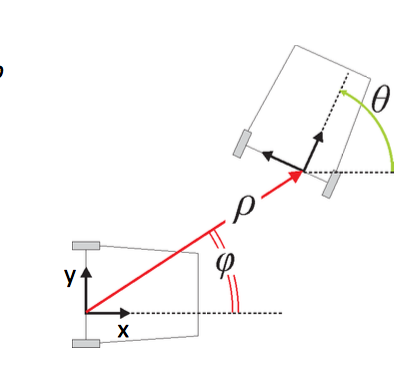
\includegraphics[scale=0.35]{pics/planar_motion}
\caption{Planar motion. \label{fig:planar_motion}}
\end{center}
\end{figure}
Let's compute the Epipolar Geometry
\begin{equation}
\begin{split}
E&=[T]_x\cdot R\\
&=\begin{pmatrix}
0&0&\rho \sin(\varphi)\\
0&0&-\rho \cos(\varphi)\\
-\rho \sin(\varphi)&\rho \cos(\varphi)&0
\end{pmatrix}\cdot \begin{pmatrix}
\cos(\theta)&-\sin(\theta)&0\\
\sin(\theta)&\cos(\theta)&0\\
0&0&1
\end{pmatrix}\\
&=\begin{pmatrix}
0&0&\rho \sin(\varphi)\\
0&0&-\rho \cos(\varphi)\\
-\rho \sin(\varphi-\theta)&\rho\cos(\varphi-\theta)&0
\end{pmatrix}.
\end{split}
\end{equation}
$E$ has 2 DoF ($\theta$, $\varphi$), because $\rho$ is the scale factor. Thus, 2 correspondences are sufficient to estimate them. Can we use less than 2 point correspondences? Yes, if we exploid wheeled vehicles with \textbf{non-holonomic} constraints. Wheeled vehicles like cars, follow locally-planar circular motion about the instantaneous Center of Rotation (ICR). Since $\varphi=\theta/2$, meaning that we have only 1 DoF. Only 1 point correspondence is needed. \textbf{This is the smallest parametrization possible and results in the most efficient algorithm for removing outliers (scaramuzza)}. This updates the problem to be
\begin{equation}
R=\begin{pmatrix}
\cos(\theta)&-\sin(\theta)&0\\
\sin(\theta)&\cos(\theta)&0\\
0&0&1
\end{pmatrix}, \qquad T=\begin{pmatrix}
\rho \cos(\frac{\theta}{2})\\
\rho \sin(\frac{\theta}{2})\\
0
\end{pmatrix}
\end{equation}
and
\begin{equation}
\begin{split}
E&=[T]_x\cdot R\\
&=\begin{pmatrix}
0&0&\rho \sin(\frac{\theta}{2})\\
0&0&-\rho \cos(\frac{\theta}{2})\\
\rho \sin(\frac{\theta}{2})&-\rho\cos(\frac{\theta}{2})&0
\end{pmatrix}.
\end{split}
\end{equation}
With the Epipolar Geometry constraint leads to
\begin{equation}
\theta = -2 \tan^{-1}\left(\frac{v_2-v_1}{u_2+u_1} \right).
\end{equation}
Up to 1000 Hz, 1-point RANSAC in only used to find the inliers. Motion is then estimated from them in 6DOF.
\begin{figure}[h!]
\begin{center}
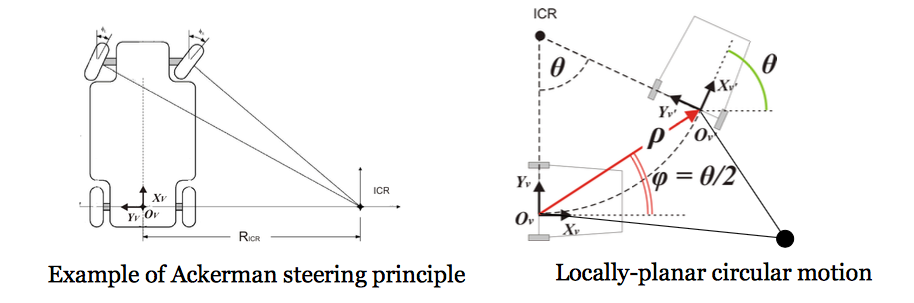
\includegraphics[scale=0.4]{pics/holonomic}
\caption{Non-holonomic. \label{fig:holonomic}}
\end{center}
\end{figure}
\newpage
\section*{Lecture 09 - Multiple View Geometry 3}
\subsection*{Bundle Adjustement (BA)}
\textbf{Nonlinear, simultaneous refinement of structure and motion (i.e. $R,T,P^i$).} It is used after linear estimation of $R$ and $T$. This, computes $R,T,P^i$ by minimizing the Sum of Squared Reprojection Errors:
\begin{equation}
(R,T,P^i)=\text{argmin}_{R,T,P^i} \sum_{i=1}^N ||p_1^i-\pi_1(P^i,C_1)||^2+||p_2^i-\pi_2(P^i,C_2)||,
\end{equation}
where $C_1,C_2$ are the \textbf{pose} of the camera in the \textbf{world frame}. This can be minimized using \textit{Lavenberg-Marquardt} (more robust than Gauss-Newton to local minima). \textbf{It is better to initialize it close to the minimum.} Same for multiple views!
\subsubsection*{Hierarchical SFM}
\begin{enumerate}
\item Extract and match features between nearby frames.
\item Identify clusters consisting of 3 nearby frames:
\item Compute SFM for the 3 frames:
\begin{itemize}
\item Compute SFM between 1 and 2 and build pointcloud.
\item Merge 3rd view running 3-point RANSAC between point cloud and 3rd view.
\end{itemize}
\item Merge clusters pairwise and refine (BA) both structure and motion. 
\end{enumerate}
Example is \textit{building Rome in one day}.
\subsubsection*{Sequential SFM}
With $n$ views. Also called Visual Odometry (VO). 
\begin{enumerate}
\item Initialize structure and motion from 2 views (\textbf{bootstrapping}).
\item For each additional view:
\begin{itemize}
\item Determine pose (localization).
\item Extend structure (i.e. extract and triangulate new features).
\item Refine both pose and structure (BA).
\end{itemize}
\end{enumerate}
\begin{enumerate}[\textbf{2D to 2D}]
\item Motion from Image feature correspondences 
\begin{itemize}
\item Both feature points $f_{k-1}$ and $f_k$ are specified in 2D.
\item The minimal-case solution involves 5-point correspondences
\item The solution is found by minimizing the reprojection error:
\begin{equation}
T_k=\begin{pmatrix}
R_{k,k-1} & t_{k,k_1}\\
0&1
\end{pmatrix}=\text{argmin}_{T_k}\sum_{i}||p_k^i-\hat{p}_{k-1}^i||^2.
\end{equation}
Popular algorithms: 8-/5-point.
\end{itemize}
\end{enumerate}
\begin{enumerate}[\textbf{3D to 2D}]
\item Motion from 3D structure and Image correspondences
\begin{itemize}
\item $f_{k-1}$ is given in 3D, $f_k$ in 2D.
\item This problem is known as \textit{camera resection} or PnP (perspective from $n$ points).
\item The minimal-case solution involves 3 \textbf{correspondences} (+1 for disambiguating the four solutions).
\item The solution is found by minimizing the reprojection error:
\begin{equation}
T_k=\begin{pmatrix}
R_{k,k-1} & t_{k,k_1}\\
0&1
\end{pmatrix}=\text{argmin}_{X^i,C_k}\sum_{i,k}||p_k^i-g(X^i,C_k)||^2.
\end{equation}
Popular algorithms: P3P.
\end{itemize}
\end{enumerate}
\begin{enumerate}[\textbf{3D to 3D}]
\item Motion from 3D-3D Point correspondences (point cloud registration).
\begin{itemize}
\item Both $f_{k-1}$ and $f_k$ are specified in 3D. To do this, it is necessary to triangulate 3D points (e.g. use a stereo camera).
\item The minimal case-solution involves \textbf{3 non collinear correspondences}
\item The solution is found by minimizing the 3D-3D euclidean distance
\begin{equation}
T_k=\begin{pmatrix}
R_{k,k-1} & t_{k,k_1}\\
0&1
\end{pmatrix}=\text{argmin}_{T_k}\sum_{i}||\tilde{X}_k^i-T_k\cdot \tilde{X}_{k-1}^i||.
\end{equation}
Popular algorithms: Arun 87, ICP, BA.
\end{itemize}
\end{enumerate}
\subsubsection*{Case Study: Monocular Visual Odometry (one camera!)}
\textbf{Bootstrapping}:
\begin{itemize}
\item Initialize structure and motion from 2 views: e.g. 8-point algorithm + RANSAC.
\item Refine structure and motion (BA)
\item How far should the frames be? If too small baseline, large depth uncertainty. If too large baseline, small depth uncertainty.
\item $\Rightarrow$ One way to avoid this consists of \textbf{skipping frames} until average uncertainty of the 3D points decreases below a certain threshold. The selected frames are called \textbf{keyframes}. In general
\begin{equation}
\frac{\text{keyframe distance}}{\text{average-depth}}>\text{threshold }(10-20\%).
\end{equation}
\end{itemize}
\textbf{Localization}
\begin{itemize}
\item Compute camera pose from known 3D-to-2D feature correspondence. 
\begin{itemize}
\item Extract correspondences by solving for $R$ and $t$ ($K$ is known).
\begin{equation}
 \lambda \cdot \begin{pmatrix}
 u\\
 v\\
 1
 \end{pmatrix}=K\cdot [R|T]\cdot \begin{pmatrix}
 X_w\\
 Y_w\\
 Z_w\\
 1
 \end{pmatrix}
 \end{equation}
\end{itemize}
 \item What is the minimal number of required point correspondences
\begin{itemize}
\item 6 for linear solution (DLT algorithm).
\item 3 for a non linear solution (P3P algorithm).
\item 3 point RANSAC.
\end{itemize}
\end{itemize}
\textbf{Extend Structure}
\begin{itemize}
\item Extract and triangulate new features.
\end{itemize}
By denoting the relative motion between adjacent keyframes as
\begin{equation}
T_k=\begin{pmatrix}
R_{k,k-1}&t_{k,k_1}\\
0&1
\end{pmatrix},
\end{equation}
we can concatenate transformations to find the full trajectory of the camera as
\begin{equation}
C_k=T_{k,k-1}\cdot C_{k-1}
\end{equation}
A non-linear refinement (BA) over the last $m$ poses (+visible structure) can be performed to get a more accurate estimate of the local trajectory. 
\subsubsection*{Loop Closure Detection (i.e. Place Recognition)}
\begin{itemize}
\item Relocalization problem: during VO, tracking can be lost (due to occlusions, low tecture, quick motion, illumination change).
\item Solution is to re-localize camera pose and continue.
\item Loop closing problem: when go back where you already have been:
\begin{itemize}
\item Loop detection: to avoid map duplication (e.g. same crossing rotated)
\item Loop correction: to compensate the accumulated drift!
\end{itemize}
\item In both cases places recognition is needed (lecture 12)
\end{itemize}
\subsubsection*{VO vs. Visual SLAM}
\begin{itemize}
\item VO: Focus on incremental estimation/\textbf{local consistency}. VO sacrifies consistency for real-time performance, without need to take into account all previous history of the camera (as SLAM does).
\item Visual VSLAM: Simultaneous Localizazion and mapping. Focus on \textbf{globally consistent} estimation. Practically VO + loop detection + graph optimization.
\end{itemize}
\subsubsection*{Feature-based Methods}
\begin{enumerate}
\item Extract and match featrues (+RANSAC)
\item Minimize Reprojection Error:
\begin{equation}
T_{k,k-1}=\text{argmin}_T\sum_{i}||u_i'-\pi(p_i)||_\Sigma^2
\end{equation}
\textbf{Good:} Large frame-to-frame motions, accuracy and efficient optimization of SFM (BA).\\
\textbf{Bad:} Slow due to costly feature extraction and matching, matching outliers (RANSAC).
\end{enumerate}
\subsubsection*{Direct Methods (all pixels)}
\begin{enumerate}
\item Minimize \textbf{photometric error}:
\begin{equation}
T_{k,k-1}=\text{argmin}_T\sum_{i}||I_k(u_i')-I_{k-1}(u_i)||_\sigma^2,
\end{equation}
where
\begin{equation}
u_i'=\pi(T\cdot (\pi^{-1}(u_i)\cdot d))
\end{equation}
\textbf{Good}: All information in the image can be exploited. Increasing camera frame-rate reduces computational cost per frame.\\
\textbf{Bad:} Limited frame to frame motion. Joint optimization of dense structures and motion too expensive.
\end{enumerate}

\subsubsection*{ORB-SLAM}
\begin{itemize}
\item Feature based:
\begin{itemize}
\item Fast corner + Oriented Rotated Brief descriptor.
\item Binary descriptor.
\item Very fast to compute and compare.
\item Minimizes reprojection error.
\end{itemize}
\item Includes:
\begin{itemize}
\item Loop closing.
\item Relocalization.
\item Final optimization.
\end{itemize}
\item Real time: 30Hz
\end{itemize}

\subsubsection*{LSD-SLAM}
\begin{itemize}
\item Direct based + Semi-dense formulation:
\begin{itemize}
\item 3D geometry represented as semi dense depth maps.
\item minimizes \textbf{photometric error}.
\item \textbf{Separately} optimizes poses and structures.
\end{itemize}
\item Includes:
\begin{itemize}
\item Loop closing.
\item Relocalization.
\item Final optimization.
\end{itemize}
\item Real time: 30Hz
\end{itemize}

\subsubsection*{DSO}
\begin{itemize}
\item Direct based + sparse formulation:
\begin{itemize}
\item 3D geometry represented as sparse large gradients.
\item Minimizes \textbf{photometric error}.
\item \textbf{Jointly} optimizes poses and structures (sliding window).
\item Incorporate photometric correction to compensate exposure time change
\end{itemize}
\item Real time: 30Hz
\end{itemize}

\subsubsection*{SVO}
\begin{itemize}
\item Direct based :
\begin{itemize}
\item Corners and edgelets.
\item Frame to frame motion estimation.
\end{itemize}
\item Feature based :
\begin{itemize}
\item Frame to Keyframe pose refinement.
\end{itemize}
\item Mapping:
\begin{itemize}
\item Probabilistic depth estimation.
\item Multi camera system
\end{itemize}
\item 400 fps on i7 laptops, 100 fps on smartphone PC
\end{itemize}
\newpage
\section*{Lecture 10 - Dense 3D Reconstruction}
For the 3D reconstruction from multiple views we assume that camera are calibrated
\begin{itemize}
\item \textbf{intrinsically} ($K$ is known for each camera), and
\item \textbf{extrinsically} ($T$ and $R$ between cameras are known).
\end{itemize}
For the multi-view stereo, we have:\\
Input: calibrated images from several viewpoints. \\
Output: 3D object dense reconstruction. 
\subsection*{Sparse Reconstruction}
We want to estimate the structure from a \textit{dense} region of pixels (hence not only from corners). The workflow is:
\begin{enumerate}
\item \textbf{Local methods}: estimate depth for every pixel independently.
\item \textbf{Global methods}: refine the depth surface as a whole by enforcing smoothness constraint.
\end{enumerate}
We use the \textbf{photometric error} (SSD): this is derived for every combination of the reference image and any further image. \textbf{IDEA}: optimal depth minizes the photometric error in all images as a function of the depth in the first image.
\subsubsection*{Aggregated Photometric Error}
The Dense reconstruction requires establishing dense correspondences. These are computed basing on the photometric error (SSD between corresponding patches of intensity values (min patch size: $1\times 1$ pixels). Pros and cons of large and small patches?
\begin{itemize}
\item Small window: Pro: more detail, Cons: more noise.
\item Large window: Pro: smoother disparity maps, Cons: less detail.
\end{itemize}
Not all te pixels can be matched reliably, due to viewpoint changes, occlusions. We take advantage of \textit{many} small baseline views, where \textit{high quality} matching is possible. Important facts:
\begin{itemize}
\item Repetitive texture shows multiple minima.
\item The aggregated photometric error for \textit{flat regions} and \textit{edges} parallel to the epipolar line show \textbf{flat valleys} (noise!).
\item For distinctive features, the aggregated photometric error has one clear minimum.
\end{itemize}
\subsubsection*{Disparity Space Image (DSI)}
For a given image point $(u,v)$ and for discrete depth hypotheses $d$, the aggregate photometric error $C(u,v,d)$ with respect to the reference image $I_r$ can be stored in a volumetric 3D grid called the \textit{Disparity Space Image (DSI)}, where each voxel (group of $u,v,d$) has value
\begin{equation}
C(u,v,d)=\sum_{k}\rho \left( \tilde{I}_k (u',v',d)-I_r(u,v)\right),
\end{equation}
where $\tilde{I}_k (u',v',d)$ is the patch of intensity values in the $k$-th image centered on the pixel $(u',v')$ corresponding to the patch $I_r(u,v)$ in the reference image $I_r$ an depth hypothesis $d$. Furthermore $rho$ is the photometric error (SSD).
\subsubsection*{Solution to depth estimation problem}
Is a function $d(u,v)$ in the DSI that satisfies:
\begin{equation}
\begin{split}
&\text{Minimum aggregated photometric error (i.e. } argmin_d C)\\
& \text{AND}\\
& \text{Piecewise smooth (global methods)}
\end{split}
\end{equation}
Interpolating while not overfitting!\\
\textbf{Global Methods:} We formulate them in terms of energy minimization. The objective is to fin a surgace $d(u,v)$ that minimizes a global energy
\begin{equation}
E(d)=\underbrace{E_d(d)}_{\text{data term}}+\underbrace{\lambda \cdot E_s(d)}_{\text{regularization term}},
\end{equation}
where 
\begin{equation}
E_d(d)=\sum_{(u,v)} C(u,v,d(u,v))
\end{equation}
and
\begin{equation}
E_s(d)=\sum_{(u,v)}\rho_d(d(u,v)-d(u+1,v))+\rho_d(d(u,v)-d(u,v+1)).
\end{equation}
$\rho_d$ is a norm (e.g. the $L_1,2$ or Huber norm). $\lambda$ controls the tradeoff data (regularization). What happens as $\lambda$ increases? Higher smoothing!
\subsubsection*{Regularized depth maps}
\begin{itemize}
\item \textbf{The regularization term} $E_s(d)$
\begin{itemize}
\item \textbf{Smooths} non smooth surfaces (result of noisy measurements) as well as discontinuities.
\item Fills the holes.
\end{itemize}
\item Popular assumption: discontinuities in intensity \textbf{coincide} with discontinuities in depth.
\item Control \textbf{smoothness penalties} according to image gradient (discrete)
\begin{equation}
\rho_d(d(u,v)-d(u+1,v))\cdot \rho_I(||I(u,v)-I(u+1,v)||)
\end{equation}
\item $\rho_I$ is some monotically \textit{decreasing} function of intensity differences: \textbf{lower} smoothness cost for \textbf{high intensity gradients}.
\end{itemize}
\subsubsection*{Choosing the stereo baseline}
What is the optimal baseline?
\begin{itemize}
\item Too small: large depth error.
\item Too large: difficult search problem.
\end{itemize}
A possible approach is \textbf{depth map fusion}.
\subsubsection*{GPGPU for Dense Reconstruction}
General Purpose Computing on Graphics Processing Unit. Perform demanding calculations on the GPU instead of the CPU. We can run processes in \textbf{parallel} on thousands of cores (CPU is optimized for serial processing). More transistor for data processing.
\begin{itemize}
\item Fast pixel processing (ray tracing, draw textures, shaded triangles,..)
\item Fast matrix/vector operations (transform vertices)
\item Programmable (shading, bump mapping)
\item Floating-point support (accurate computations)
\item Deep learning.
\end{itemize}
And
\begin{itemize}
\item \textbf{Image processing}
\begin{itemize}
\item Filtering and feature extractions (e.g. convolutions)
\item Warping (e.g. epipolar rectification, homography).
\end{itemize}
\item \textbf{Multiple-view geometry}
\begin{itemize}
\item Search for dense correspondences (pixel wise operations, matrix and vector operations (epipolar geometry).
\item Aggregated photometric error.
\end{itemize}
\item \textbf{Global Optimation}
\item Variational methods (i.e. regularization (smoothing)) (divergence computation)
\end{itemize}
Typically on consumer hardware: 1024 threads per multiprocessor, 30 multiprocessors: 30000 threads. CPU with 4 cores which supports 32 threads. High arithmetic intensity.\\
Have a look at Scaramuzza work!
\newpage
\section*{Lecture 11 - Tracking}
\subsection*{Point Tracking}
\textbf{Problem:} Given two images, estimate the motion of a pixel from image $I_0$ to image $I_1$. Two approaches exist, depending on the amount of motion between the frames:
\begin{itemize}
\item \textbf{Block-based methods}
\item \textbf{Differential methods}
\end{itemize}
\subsubsection*{Block-based methods}
\begin{itemize}
\item Search for the corresponding patch in a \textit{neighborhood} around the point.
\item Use SSD, SAD, NCC to search for corresponding patches in a local neighborhood of the point. The search region usially is a $D\times D$ squared patches.
\end{itemize}
\subsubsection*{Differential Methods}
\begin{itemize}
\item Look at the local brightness changes at the \textbf{same} location. \textbf{NO patch shift} is performed. (centered in the same point!)
\end{itemize}
\subsubsection*{Spatial Coherency}
We assume that all the pixels in the patch undergo the same motion (same $u$ and $v$). Also, assume that the time interval between the two images $I_0$ and $I_1$ is small. We want to find the motion vector $(u,v)$ that minimizes the Sum of Squared Differences (SSD)
\begin{equation}
\begin{split}
SSD&=\sum(I_0(x,y)-I_1(x+u,y+v))^2 \\
&\approx \sum(I_0(x,y)-I_1(x,y)-I_x\cdot u -I_y \cdot v)^2\\
&=\sum(\Delta I-I_x\cdot u - I_y \cdot v)^2,
\end{split}
\end{equation}
which is a simple quadratic function in two variables $(u,v)$.
\subsubsection*{Motion Vector}
To minimize the $E$, we differentiate with respect to $(u,v)$ and equate to 0.
\begin{equation}
\begin{split}
\frac{\partial E}{\partial u}&=0 \Rightarrow -2 \sum(\Delta I-I_x\cdot u - I_y \cdot v)=0\\
\frac{\partial E}{\partial v}&=0 \Rightarrow -2 \sum(\Delta I-I_x\cdot u - I_y \cdot v)=0
\end{split}
\end{equation}
Linear system of two equations in two unknowns. We can write this in matrix form
\begin{equation}
\begin{split}
\begin{pmatrix}
\sum I_xI_x & \sum I_x I_y\\
\sum I_xI_y & \sum I_y I_y
\end{pmatrix} \cdot \begin{pmatrix}
u\\ v 
 \end{pmatrix}&= \begin{pmatrix}
 \sum I_x \cdot \Delta I\\
  \sum I_y \cdot \Delta I\\
 \end{pmatrix}\\
 \begin{pmatrix}
u\\ v 
 \end{pmatrix}&=\begin{pmatrix}
\sum I_xI_x & \sum I_x I_y\\
\sum I_xI_y & \sum I_y I_y
\end{pmatrix} ^{-1}\cdot \begin{pmatrix}
 \sum I_x \cdot \Delta I\\
  \sum I_y \cdot \Delta I\\
 \end{pmatrix}
 \end{split}
\end{equation}
\newpage
\section*{Lecture 13 - Visual Inertial Fusion}
\subsection*{Pose Graph Optimization}
So far we assumed that the transformations are between consecutive frames, but transformation can be computed also between non adjacent frames $T_{ij}$ (e.g. when features from previous keyframes are still observed). They can be used as additional constraints to improve cameras poses by minimizing the following:
\begin{equation}
C_k=\text{argmin}_{c_k} \sum_{i} \sum_{j} ||C_i-C_j\cdot T_{ij}||^2
\end{equation}
\begin{itemize}
\item For efficiency, only the last $m$ keyframes are used.
\item Gauss-Newton or Levenber-Marquadt are typically used to minimize it. For large graphs, there are open source things.
\end{itemize}
\begin{figure}[h!]
\begin{center}
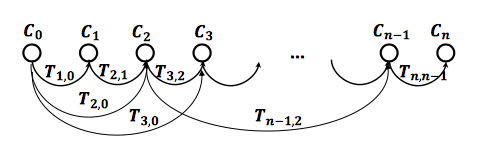
\includegraphics[scale=0.5]{pics/pose}
\caption{Pose graph optimization.}
\end{center}
\end{figure}
\subsection*{Bundle Adjustment (BA)}
This incorporates the knowledge of landmarks (3D points).  
\begin{equation}
X^i,C_k=\text{argmin}_{X^i,C_k} \sum_{i} \sum_{k}\rho \left( p_k^i-\pi(X^i,C_k)\right).
\end{equation}
Outliers are a problem, how can we penalize them? In order to penalize wrong matches, we can juse the Huber or Turkey cost.
\begin{equation}
\begin{split}
\text{\textbf{Huber}} \qquad \rho(x)&=\begin{cases}
x^2, &if \ |x|\leq k\\
k\cdot (2|x|-k)& if \ |x| \geq k \text{ linear}
\end{cases}\\
\text{\textbf{Tukey}} \qquad \rho(x)&=\begin{cases}
\alpha^2&if \ |x|\geq \alpha \\
\alpha^2 \cdot \left(1-(1-(\frac{x}{\alpha})^2)^3 \right)&if \ |x|\leq \alpha.
\end{cases}
\end{split}
\end{equation}

\subsubsection*{Bundle Adjustment vs Pose-graph Optimization}
\begin{itemize}
\item BA is more precise than pose-graph optimization because it adds additional constraints (landmark constraints).
\item But \textbf{more costly}: $O((qM+lN)^3)$ with $M$ and $N$ being the number of points and camera poses and $q$ and $l$ the number of parameters for points and camera poses. Workarounds are
\begin{itemize}
\item A small window size limits the number of parameters for the optimization and thus makes real-time bundle adjustment possible.
\item It is possible to reduce the computational complexity by just optimizing the camera parameters and keeping the 3D landmarks fixed, e.g. \textbf{freeze the 3D points and adjust the poses}
\end{itemize}
\end{itemize}
\begin{figure}[tbh]
\begin{center}
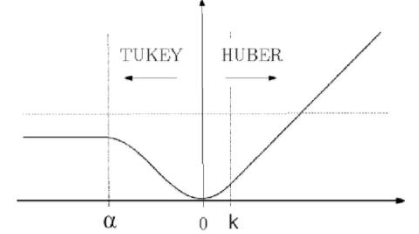
\includegraphics[scale=0.5]{pics/tukey}
\caption{Tukey vs. Huber norm.}
\end{center}
\end{figure}

\begin{figure}[tbh]
\begin{center}
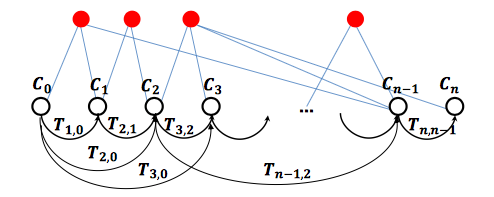
\includegraphics[scale=0.5]{pics/bundle}
\caption{Bundle Adjustment.}
\end{center}
\end{figure}
\subsection*{IMUs}
Inertial Mesaurement Unit. Measures \textbf{angular velocity} and \textbf{linear accelerations}. 
\begin{itemize}
\item Mechanical: spring/damper system.
\item Optical: Phase shift projected laser beams is proportional to angular velocity.
\item MEMS (accelerometer): a spring-like structure connects the device to a seismic mass vibrating in a capacitive divider. A capacitive divider converts the displacement of the seismic mass into an electric signal. Damping is created by the gas sealed in the device.
\item MEMS (gyroscopes): measure the Coriolis forces acting on MEMS vibrating structures. Their working principle is similar to the haltere of a fly. Have a look!
\end{itemize}
\subsubsection*{Why IMU?}
\begin{itemize}
\item Monocular vision is scale ambiguous.
\item Pure vision is not robust enough (Tesla accident):
\begin{itemize}
\item Low texture.
\item High dynamic range.
\item High speed motion.
\end{itemize}
\end{itemize}
\subsubsection*{Why not just IMU?}
Pure IMU integration will lead to large drift (especially cheap IMUs). Integration of angular velocity to get orientation: error \textbf{proportional to $t$}. Double integration to get position: if there is a bias in acceleration, the error of position is \textbf{proportional to $t^2$.} The actually position error also depends on the error of orientation.
\subsubsection*{Why visual inertial fusion?}
\begin{itemize}
\item \textbf{Cameras}
\begin{enumerate}[+]
\item Precise in slow motion.
\item Rich information for other purposes
\end{enumerate}
\begin{enumerate}[-]
\item Limited output rate ($\sim 100 Hz$)
\item Scale ambiguity in monocular setup.
\item Lack of robustness
\end{enumerate}
\item \textbf{IMU}
\begin{enumerate}[+]
\item Robust.
\item High output rate ($\sim 1000 Hz$).
\item Accurate at high acceleration.
\end{enumerate}
\begin{enumerate}[-]
\item Large relative uncertainty when at low acceleration/angular velocity.
\item Ambiguity in gravity / acceleration.
\end{enumerate}
\end{itemize}
Together, they can work for state estimation: loop detection and loop closure.
\subsubsection*{IMU: Measurement Model}
\begin{equation}
\begin{split}
\tilde{\omega}_{WB}^B(t)&=\omega_{WB}^B(t)+b^g(t)+n^g(t)\\
\tilde{a}_{WB}^B(t)&=R_{BW}(t)\cdot \left(a_{WB}^W(t)-g^W \right) + b^a(t)+n^a(t)
\end{split}
\end{equation}




\end{document}
